\documentclass[a4paper,11pt,twoside]{book}
\usepackage[T1]{fontenc}
\usepackage[utf8]{inputenc}
\usepackage[french]{babel}
\usepackage{color}
\usepackage{graphicx}
\usepackage{amsthm}
% Evite les erreurs de justification
% http://tex.stackexchange.com/questions/174903/justified-text-extending-beyond-margin
\usepackage{microtype}
\usepackage{adjustbox}
\usepackage{arydshln,tabulary,multirow,booktabs,array}
\usepackage{url}

\usepackage{tikz}
\usetikzlibrary{mindmap,trees}
\tikzset{concept/.append style={fill={none}}}
%\tikzset{
%  set angles for level/.style={level #1/.append style={sibling angle=360/\the\tikznumberofchildren}},
%  level/.append style={set angles for level=#1}% solution 1
%}

%\usepackage{verbatim}

\newtheorem{definition}{Definition}

\begin{document}
%    \begin{titlepage}
\begin{center}
\noindent {\large \textbf{CentraleSupélec}} \\
\vspace*{0.3cm}
\noindent {\LARGE \textbf{ÉCOLE DOCTORALE STIC}} \\
\noindent \textbf{SCIENCES ET TECHNOLOGIES DE L'INFORMATION \\ ET DE LA COMMUNICATION} \\
\vspace*{0.5cm}
\noindent \Huge \textbf{T H È S E} \\
\vspace*{0.3cm}
\noindent \large {pour obtenir le titre de} \\
\vspace*{0.3cm}
\noindent \LARGE \textbf{Docteur en Sciences} \\
\vspace*{0.3cm}
\noindent \Large de CentraleSupélec \\
\noindent \Large \textbf{Mention : \textsc{Informatique}}\\
\vspace*{0.4cm}
\noindent \large {Présentée et soutenue par\\}
\noindent \LARGE Rachida \textsc{Seghiri} \\
\vspace*{0.8cm}
\noindent {\Huge \textbf{Simulation des SI des Smart Grids (à revoir)}} \\
\vspace*{0.8cm}
\noindent \Large Thèse dirigée par Frédéric \textsc{Boulanger} \\
\vspace*{0.2cm}
\noindent \Large préparée à EDF R&D, Projet \textsc{Pomme} \\
\vspace*{0.2cm}
\noindent \large   \\
\vspace*{0.5cm}
\end{center}
%\noindent \large \textbf{Jury :} \\
%\begin{center}
%\noindent \large 
%\begin{tabular}{llcl}
%      \textit{Rapporteurs :}	&  		&  &  \\
%				&  \textsc{Collins}		& - & McGill University\\
%      \textit{Directeur :}	& Grégoire \textsc{Malandain}		& - & INRIA (Asclepios)\\
%      \textit{Président :}	& Nicholas \textsc{Ayache}		& - & INRIA (Asclepios)\\
%      \textit{Examinateurs :}   & Pierre-Yves \textsc{Bondiau}          & - & Centre Antoine Lacassagne (Nice)\\
%      				& Guido \textsc{Gerig}			& - & University of North Carolina\\
%      				& Vincent \textsc{Grégoire}		& - & Université Catholique de Louvain\\
%      \textit{Invité :}		& Hanna \textsc{Kafrouni}		& - & DOSISoft S.A.
%\end{tabular}
%\end{center}
\end{titlepage}
\sloppy

\titlepage

    \cleardoublepage
%    \section*{Remerciements}
    \tableofcontents
    \mainmatter
%    \chapter{État de l'art}
\label{chap:Etat de l'art}

\section{Architecture d'Entreprise}

\subsection{Terminologie}

\textbf{Système d'Information (SI)}

Selon Robert Reix, le SI est «~un ensemble organisé de ressources : matériel, 
logiciel, personnel, données, procédures permettant d'acquérir, de traiter, de 
stocker des informations (sous forme de donnée, textes, images, sons, etc.) dans 
et entre des organisations.~»

Nous adoptons cette définition car elle a l'avantage de ne pas réduire le SI 
d'une organisation à son système informatique. Ce dernier est constitué de 
l'ensemble du patrimoine matériel (hardware) et applicatif (software) de la dite 
organisation et a pour objectif d'automatiser le traitement de l'information. 
Nous adoptons l'acronyme IT (\textit{Information Technologies}) pour le 
différencier du SI.

On suppose souvent que les SI sont totalement informatisés et c'est une des raisons qui mènent à confondre SI et IT. Cependant, le SI comprend non seulement le système informatique mais aussi les ressources humaines (partenaires, personnel, etc.) et immatérielles (procédures de gestion, savoir-faire métier, etc.).



\textbf{Architecture d'Entreprise  (AE)}

Frank Armour définit le terme «~architecture~» de manière simple \cite{armour1999bigpicture} : il s'agit de la description d'un ensemble de composants et de leurs relations.

S'agissant du terme «~entrerprise~», Scott Bernard 
\cite{bernard2012introduction} y réfère comme une
organisation ou une sous-partie d'une organisation qui poursuit des objectifs communs, en s'appuyant sur les mêmes processus et en utilisant les mêmes ressources. Une entreprise peut être publique ou privée, avoir ou pas un but lucratif. 

Dans un premier temps, nous introduisons  l'architecture d'entreprise en utilisant l'analogie avec l'architecture du bâtiment. En effet, construire une maison en 
procédant chambre par chambre sans plan d'architecture général peut mener à un résultat peu probant. De même, le développement d'une organisation, sans architecture de référence globale et préalable, risque de mener à une duplication de ses ressources et altère par conséquent son efficacité \cite{bernard2012introduction}.

Dans la littérature, il existe une multitude de définitions de l'architecture d'entreprise émanant du aussi bien du monde académique que du monde industriel. 
Néanmoins, aucune définition n'a été universellement adoptée \cite{mentz2012comparison} \cite{ranganathan2005enterprise}. Ce manque de consensus est certainement du à la nature intrinsèque de l'architecture d'entreprise. En effet, cette dernière est 
régie par un ensemble de préceptes et de bonnes pratiques que chacun reste libre d'adapter à son propre besoin. 

Toutefois, il est possible d'identifier un thème commun à toutes les définitions proposées : l'architecture d'entreprise décrit les composants interdépendants d'une organisation et guide leurs évolutions \cite{lapalme2012three}. En revanche, le 
\textit{périmètre} de cette description ainsi que les \textit{préoccupations} adressées diffèrent d'une définition à l'autre.

S'agissant du \textit{périmètre} des définitions existantes, le terme 
«~entreprise~» peut couvrir uniquement l'IT à l'échelle de l'entreprise ou s'entendre à tous les composants humains, stratégiques, économiques et techniques qui la 
constituent. Les \textit{préoccupations} sous-jacentes à l'activité d'architecture peuvent, quant à elles, couvrir des finalités allant de l'optimisation des investissements dans l'infrastructure technique jusqu'à 
l'implémentation de la stratégie de l'entreprise en passant par l'alignement métier/IT. 

Partant de ce constat, James Lapalme identifie trois écoles de pensée pour l'AE 
\cite{lapalme2012three} : l'architecture de l'IT d'entreprise, l'intégration 
d'entreprise et l'entreprise dans son environnement. Chacune de ces écoles a son propre système de croyance (devise, préoccupations et objectifs, principes et postulats).


%\textcolor{red}{Le terme "système de croyances" est vraisemblablement emprunté à 
%la  sociologie, j'aime bien l'idée d'utiliser d'autres disciplines pas forcément 
%directement mais Lapalme ne fait pas du tout la référence à la sociologie en 
%parlant de belief system. J'ai une amie qui a un master en socio je peux lui 
%demander une petite référence pour définir exactement ce qu'est un système de 
%croyances. En lisant la préface de Zachman dans le livre de Scott Bernard, on y 
%entrevoit clairement une problématique de catégorie de gens qui croient que la 
%clé de l'architecture c'est la technologie sans  tenir compte des problématiques 
%métier. à voir donc. Au pire je supprime simplement le terme «~système de croyances~» mais je trouve ça dommage parce que ça explique pas mal de choses.}

Il est important de noter que cette catégorisation est épurée, voire idéalisée, dans la mesure où une majorité d'auteurs gravite autour d'une école plutôt que 
de complètement rentrer dans une seule catégorie. 

Le tableau 1 fait correspondre à chacune de ces écoles, leurs périmètres ainsi que leurs préoccupations respectives. 



\newlength{\bigtable}
\setlength{\bigtable}{1.3\textwidth}
\setlength{\dashlinedash}{0.5pt}
\setlength{\dashlinegap}{1pt}
\setlength{\arrayrulewidth}{0.5pt}
\begin{adjustbox}{width=\bigtable,center}
    \newlength{\mycolumnwidth}
    \setlength{\mycolumnwidth}{\dimexpr0.28\bigtable-2\tabcolsep\relax}
    \newlength{\myfirstcolumn}
    \setlength{\myfirstcolumn}{\dimexpr0.16\bigtable-2\tabcolsep\relax}
    \scriptsize
    \begin{tabulary}{\bigtable}{@{}>{\bfseries}p{\myfirstcolumn}p{\mycolumnwidth}p{\mycolumnwidth}p{\mycolumnwidth}@{}}
        %  --------------------------------------------------------------------
        \toprule
        & \centering\textbf{Enterprise IT Architecting} \
        & \centering\textbf{Enterprise Integration} \
		& \centering\textbf{Enterprise Ecological\newline Adaptation}\
        \tabularnewline\midrule
        %  --------------------------------------------------------------------
        \multirow{1}{\myfirstcolumn}{Devise} \
        & L'architecture d'entreprise raccorde l'IT au métier de l'entreprise \
        & L'architecture d'entreprise lie la stratégie et son exécution \
        & L'architecture d'entreprise est un moyen d'innovation organisationnelle et une garantie de durabilité  \
        \tabularnewline\midrule
        %  --------------------------------------------------------------------
        \multirow{3}{\myfirstcolumn}{Objectifs et préoccupations} \
        & Planifier l'IT et en optimiser les coûts \
        & Implémenter efficacement la stratégie de l'entreprise \
        & Adapter et innover \
        \tabularnewline\addlinespace\cdashline{2-4}\addlinespace%\tabularnewline\cmidrule{2-4}
        & Appuyer le métier \
        & Assurer la cohésion de l'organisation \
        & Assurer la cohésion de l'organisation \\
        \tabularnewline\addlinespace\cdashline{2-4}\addlinespace%\tabularnewline\cmidrule{2-4}
        & \
        & \
        & Encourager la co-évolution entre l'entreprise et son environnement \
        \tabularnewline\midrule
        %  --------------------------------------------------------------------
        \multirow{4}{\myfirstcolumn}[4pt]{Principes et postulats} \
        & Appliquer une approche réductionniste \
        & Appliquer une approche holistique \
        & Appliquer une approche holistique \
        \tabularnewline\addlinespace\cdashline{2-4}\addlinespace%\tabularnewline\cmidrule{2-4}
        & Ne pas remettre en question la stratégie et les objectifs métier \
        & Ne pas remettre en question la stratégie et les objectifs métier \
        & Créer la stratégie de l'entreprise est une priorité \
        \tabularnewline\addlinespace\cdashline{2-4}\addlinespace%\tabularnewline\cmidrule{2-4}
        & Concevoir les composants de l'organisation de manière indépendante \
        & Concevoir les différents aspects de l'entreprise de manière intégrative\
        & Concevoir les différents aspects de l'entreprise de manière intégrative\
        \tabularnewline\addlinespace\cdashline{2-4}\addlinespace%\tabularnewline\cmidrule{2-4}
        & Ne pas se préoccuper des aspects non IT \
        & Tenir compte de l'environnement comme source de changement \
        & L'environnement peut être transformé \
        \tabularnewline\midrule
%        %  --------------------------------------------------------------------
%        \multirow{3}{\myfirstcolumn}[9pt]{Skills} \
%        & Have techinal competence and engineering knowledge \
%        & Facilitate small-group collaboration \
%        & Foster dialogue \
%        \tabularnewline\addlinespace\cdashline{2-4}\addlinespace%\tabularnewline\cmidrule{2-4}
%        & \
%        & Apply systems thinking \
%        & Apply system and system-in-environment thinking \
%        \tabularnewline\addlinespace\cdashline{2-4}\addlinespace%\tabularnewline\cmidrule{2-4}
%        & \
%        & \
%        & Facilitate larger-groups collaboration \
%        \tabularnewline\bottomrule
    \end{tabulary}
\end{adjustbox}

\\

%Dans ce contexte, l'Architecture d'Entreprise est une discipline qui a pour 
%vocation de décrire une telle organisation en offrant une vue générale et 
%homogène de son métier, de son patrimoine applicatif et de infrastructure 
%technique ainsi que leur évolution pour en faciliter l'analyse par biais d'un 
%ensemble cohérents de principes, méthodes et modèles 
%\cite{lankhorst2009enterprise}.






%C'est ce qui a amené Dankova à classifier les définitions existantes 
%selon l'aspect sur lequel leurs auteurs décident de mettre l'accent. Il en 
%ressort quatre catégories de définition : 
%\begin{itemize}
%\item Planification et conception
%
%L'AE représente un plan descriptif de la structure d'une organisation avec ses 
%différents composants et les relations entre ces composants. La but de ce plan 
%étant de trouver le moyen le plus efficace pour que l'entreprise  son objectif.
%\item Planification et conception
%
%L'AE est conçue comme un ensemble de principes, de règles et de modèles que 
%doit 
%respecter l'implémentation de l'entreprise ne partant du métier jusqu'à 
%l'infrastructure technique.
%\item ICT
%
%\textcolor{red}{to do}
%\item Métier
%
%\textcolor{red}{to do}
%\end{itemize}

En construisant cette taxonomie des différentes écoles de pensée existante, Lapalme insiste sur le fait que ces écoles se sont établies par héritage. En effet, l'\textit{Enterprise Ecological Adaptation} hérite de l'\textit{Enterprise Integration}, qui elle même hérite l'\textit{Enterprise IT architecting}. Cependant, cet l'héritage implique une transcendance. En effet, il existe des différences fondamentales entre ces différentes écoles. Par exemple, si l'l'\textit{Enterprise IT architecting} applique une approche réductionniste 
Il est important de noter que le terme architecture d'entreprise peut prêter à confusion car il est à la fois utilisé pour désigner (1) l'activité de conception d'une architecture i.e. la description des éléments composant l'organisation en question et leurs relations mais aussi (2) l'ensemble des artefacts résultant de cette activité. 
Pour éviter toute confusion, nous désignons l'activité de conception par le terme architecture d'entreprise et résultat de cette activité comme étant l'architecture de l'entreprise.



\subsection{De l'architecture IT vers l'Architecture de l'Entreprise dans son environnement}

L'architecture d'entreprise est ancrée dans l'architecture de systèmes 
informatique \cite{kappelman2008enterprise}. Ensuite, elle a évolué vers une 
architecture qui comprends l'IT mais aussi les aspects métier de l'entreprise 
\cite{winter2006essential}  jusqu'à adresser l'ensemble de l'entreprise en 
intégrant la stratégie de l'entreprise et ses processus décisionnels 
\cite{ross2006enterprise} allant même jusqu'à aborder l'environnement dans 
lequel elle évolue.

En effet, l'origine de l'EA\footnote{D'après Scott Bernard 
\cite{bernard2012introduction}, le terme Architecture d'Entreprise a fait sa 
première apparition dans le livre de Steven Spewak intitulé "Enterprise 
Archietcture Planning : developing a blueprint for data, applications and 
technology" \cite{spewak1993enterprise}.} remonte au travaux de Zachman, souvent 
considérés comme précurseurs. Il y propose un cadre d'architecture pour l'IT 
\cite{zachman1987framework}.

De ce fait, l'Architecture d'Entreprise (AE) a initialement été conçue pour 
optimiser la 
gestion du patrimoine applicatif et de l'infrastructure technique d'une  
entreprise. À ses débuts, l'AE se 
focalise sur des artefacts purement IT (data, logiciels, équipements) pour 
rationaliser les l'utilisation des ressources informatiques 
\cite{winter2006essential} tout en répondant aux besoins métier de l'entreprise. 
L'AE est alors guidée par les pratiques d'ingénierie logicielle. \textcolor{blue}{Ecole 1} 
 

Cependant, le rôle de plus en plus prégnants de l'IT et son impact sur le c\oe{}ur de métier des organisations ainsi que l'accroissement de sa complexité 
\cite{ranganathan2005enterprise} ont fait de l'architecture de l'IT d'une 
entreprise une problématique inhérente à l'architecture de l'ensemble de 
l'entreprise. Ainsi, l'AE a commencé à intégrer des aspects métier tels que les 
objectifs de l'organisation, les processus métier, les indicateurs de 
performances \cite{winter2006essential}. En intégrant ainsi des problématiques 
métier, L'AE ne relève plus de l'architecture IT mais de l'architecture du SI 
dans son ensemble.

Pour Scott Bernard, l'AE doit même aller plus loin en intégrant la stratégie de 
l'entreprise \cite{bernard2012introduction} dans son champs de discipline pour 
profiter pleinement de l'ensemble des ressources de l'entreprise (métier, IT, 
humaines, etc.). Ainsi, le terme "~entreprise~" implique une vue stratégique de 
haut niveau de l'organisation dans son ensemble. Quand au terme 
"~architecture~", il sous-entend la mise en place d'un cadre structuré pour 
l'analyse, le planning, et le développement de toutes les ressources dont 
dispose l'organisation. \textcolor{blue}{Ecole 2} 

Enfin, pour certains auteurs, l'entreprise s'inscrit dans un environnement 
particulier, souvent inconstant \cite{lapalme2012three}. Par conséquent, l'AE 
doit inclure les relations de l'entreprise avec son environnement pour en 
déterminer les impacts et faciliter ainsi les processus d'adaptation  et 
d'innovation. \textcolor{blue}{Ecole 2}


\textcolor{blue}{Schéma évolution de l'AE dans les différentes écoles}.  



%L'évolution de l'AE fait émerger plusieurs écoles de pensée chacune ayant sa 
propre vision de l'AE, ses périmètres, ses limitations et ses postulats.

  
\subsection{Avantages de l'Architecture d'Entreprise}
L'AE est un outil efficace pour organiser et structurer les informations à 
l'échelle de l'organisation en fournissant les détails appropriés à chacune des 
parties prenantes ainsi que l'ensemble des principes et des recommandations pour 
construire un SI aussi bien aligné au besoins métier qu'évolutif. Les avantages 
potentiels que procurent l'AE sont autant liés à l'IT qu'au métier de 
l'organisation \cite{ross2005understanding}.

Le tableau (ref) résume ces avantages \cite{shah2007frameworks} : 
(tableau à faire). 
Avantages / Description
pour l'IT
Gestion de la complexité / Facilité l'orientation et la coordination des projets 
liés à l'IT. Décrire les interdépendances des systèmes de manières exploitable.
Supervision des ressources techniques / Identifier et supprimer les redondances.
Gestion de la connaissance /  Gérer et partager les connaissances concernant 
l'IT de manière à ce qu'elles soient visualisables à différents niveaux 
d'abstraction par toutes les parties prenantes 
Visibilité sur l'IT / les ressources IT sont mieux alignés avec les stratégies 
métier et plus réactives
pour le métier 
Réduction de l'impact du au changement de personnel / Capturer les connaissances 
des employés et des consultants. 
Adaptabilité rapide /  Facilité l'accès aux informations nécessaires pour 
remplacer des composants
Amélioration des procédures opérationnelles / Modéliser et mieux appréhender les 
processus métier. Examiner les processus et faciliter leur réingénierie  .
Prise de décision / Représenter les composants de l'organisation  en offrant une 
vision à la fois globale et adaptée au décideur facilite la prise de décision.




%L'Architecture d'Entreprise (AE) est un moyen efficace pour capturer les 
composants d'une entreprise dans ses états courants et désirés.  

\subsection{AE et modélisation}

Quelle qu'en soit l'école, l'architecture d'entreprise reste une tâche complexe 
\cite{steen2004supporting} en raison du grand nombre de parties prenantes 
impliquées, chacune ayant des préoccupations et des systèmes de notation propres 
dépendant de leur domaine d'expertise et des responsabilités qui leur incombent.

L'AE est donc sensée capturer une grandes variété de composants et il est 
d'autant plus difficile des les représenter dans un seul et unique modèle. 
Faisons le parallèle avec l'architecture d'une vile. Par exemple, utiliser un 
seul plan pour représenter à la fois les réseaux de transports, d'électricité, 
de gaz et d'eau potable ainsi que les rues et les bâtiments d'une ville rend le 
plan illisible par tous les acteurs concernés.

Il en est de même pour l'AE. La nature mutli-facettes inhérente à l'architecture 
d'une entreprise rend inappropriée toute approche monolithique 
\cite{armour1999bigpicture}. En effet, un analyste métier est concerné par les 
processus et les fonction métier alors qu'un administrateur de base de données 
est concerné par les données manipulées. Par conséquent, la plupart des 
framework d'AE adoptent une approche par points de vue.

Les approches orientées par de vue ont d'abord été élaborées pour la 
spécification des besoins en ingénierie logicielle \cite{mullery1979core}. Les 
chercheurs s'intéressent alors aux systèmes à "~perspectives multiples~" 
\cite{finkelstein1992viewpoints} \cite{kotonya1996requirements} 
\cite{nuseibeh1994multi} \cite{meyers1993representing}. 

Ces travaux précurseurs contribuent à l'émergence de plusieurs normes proposant 
des cadres d'architecture orientés points de vue pour les systèmes logiciels. Il 
en est ainsi de la norme IEEE-1471(ref), du standard RM-ODP (réf) (Reference 
Model of Open Distributed Processing) ou encore du standard MDA (Model Driven 
Architecture) (réf).

Pour la norme IEEE\-1471 les concepts de vue et de points de vue sont essentiels. 
Une vue est définie comme étant une représentation du système selon une certaine 
perspective à laquelle est associée un ensemble de préoccupations. Les vues 
permettent ainsi de séparer les préoccupations des différentes parties 
prenantes. Un point de vue est quand un lui un template pour la création de 
vues. Il formalise les objectifs des parties prenantes concernées par la vue 
ainsi que les techniques qui permettent de la créer et de l'analyser. Pour 
définir un point de vue, la norme IEEE\-1471 exigent de spécifier les attributs 
suivant :
\begin{itemize}
\item le nom du point de vue
\item la partie prenante ciblée
\item les préoccupations de celle-ci
\item le langage, les techniques de modélisation ou encore les méthodes 
d'analyse à utiliser pour la création de la vue. 
\end{itemize}


Ainsi, l'approche orientée points de vue pour gérer la complexité des 
architectures est déjà bien établie en ingénierie logicielle 
\cite{steen2004supporting}. L'AE trouvant ses origines dans l'architecture IT 
(cf. section précédente), de nombreux cadres d'architecture d'entreprise 
recourent cette approche en transférant les concepts développés dans 
l'architecture IT au domaine de l'AE.

Ces frameworks n'utilisent pas les mêmes points de vue~: leur nombre, leur nom 
ainsi que les préoccupations qu'ils adressent peuvent variés. Cependant, ces 
frameworks ont souvent en commun les points de vue suivants :
\begin{itemize}
\item point de vue métier \textcolor{red}{to do}
\item point de vue information \textcolor{red}{to do}
\item point de vue fonctionnel \textcolor{red}{to do}
\item point de vue applicatif \textcolor{red}{to do}
\item point de vue technique \textcolor{red}{to do}.
\end{itemize} 
En outre, ces frameworks organisent hiérarchiquement les différentes vues en 
appliquant \emph{«3~IT follows business~»} comme principe : commencer par le 
point de vue métier et le dériver progressivement jusqu'à l'infrastructure 
technique déployée en passant par les fonctions et les applications 
\cite{winter2006essential}.



%%%%%Anicienne version%%%%%%%%%
Quelle qu'en soit l'école, l'architecture d'entreprise tente de capturer les 
composants d'une organisation mais bien souvent la réalité d'u 
Une représentation appropriée d'une telle architecture reflète donc les besoins 
des acteurs (décideur, expert du domaine métier, architecte fonctionnel, 
architecte technique, etc.) en explicitant les informations manipulées.  
\\Étant donnée la complexité des SI actuels, en particulier ceux des Smart 
Grids, et la multitude des acteurs concernés, une vision monolithique est 
inappropriée à la construction de SI évolutifs et adaptés aux différents 
acteurs.
\\Plusieurs cadres d'architecture adoptent une approche par points de vue. Un 
point de vue formalise la perspective d'un acteur particulier du SI. Une vue est 
conforme à ce point de vue. C'est le cas de RM-ODP \cite{raymond1995reference}, 
de TOGAF \footnote{The Open Group Architecture Framework} 
\footnote{www.opengroup.fr/togaf}, de la méthode « 4+1 » de Kruchten 
\cite{kruchten19954+} ainsi que de la norme ISO/IEC/IEEE 
42010\footnote{http://www.iso-architecture.org/}. Le SGAM\footnote{Smart Grid 
Archietcture Model} \cite{uslar2012standardization} adresse l'architecture du 
Smart Grid en englobant les trois domaines : SI, réseau électrique et réseau de 
télécommunication. 
\\En outre, ces frameworks organisent hiérarchiquement les différentes vues en 
appliquant \emph{« IT follows business »} comme principe : commencer par le 
point de vue métier et le dériver progressivement jusqu'à l'infrastructure 
technique déployée en passant par les fonctions et les applications 
\cite{winter2006essential}. 
Souvent, ces cadres d'architecture distinguent quatre points de vue principaux~:
\begin{description}
\item[Point de vue métier]  : ce point de vue reflète la vision métier. On y 
retrouve les objectifs métier de l'entreprise, les processus, ainsi que les 
acteurs~;
\item[Point de vue fonctionnel] : ce point de vue organise le SI en blocs 
fonctionnels de manière à garantir son évolutivité tout en répondant aux besoins 
métier de l'entreprise. A l'échelle du SI d'une entreprise, cette structuration 
devient vite complexe à cause du caractère étendu et transverse des processus 
métier impactés~;
\item[Point de vue applicatif] : ce point de vue structure le SI en blocs 
applicatifs, chacun implantant un ou plusieurs blocs fonctionnels~;
\item[Point de vue technique] : ce point de vue correspond à l'infrastructure 
technique du SI (matériel informatique et réseaux télécom).
\end{description}




\section{Ingénierie Dirigée par les Modèles}

L'Ingénierie Dirigée par les Modèles (IDM) est née du constat que le paradigme 
du « tout est objet », prôné dans les années 1980, a atteint ses limites avec ce 
début de siècle \cite{greenfield2004software}. En effet, face à la croissance de 
la complexité des systèmes logiciels, au coût de la main d'œuvre et de 
maintenance, une approche centrée sur le code, jugé alors seul représentant 
fiable du système, suscitait de moins en moins l'adhésion des industriels et du 
milieu académique. 

Partant de ce constat, l'Object Management Group (OMG) a proposé en novembre 
2000, l'approche MDA (Model Driven Architecture) qui s'inscrit dans le cadre 
plus général de l'IDM et se réalise autour d'un certain nombre de standards tels 
qu'UML, MOF, XML, QVT, etc. Le monde de la recherche s'y est aussitôt intéressé 
pour dégager les principes fondamentaux de l'IDM 
\cite{bezivin2001towards}\cite{kent2002model} \cite{de2002using} et déjouer le 
piège des définitions parfois trop floues qui prêtent à confusion entre les 
concepts liés aux paradigmes d'objet et de modèle \cite{bezivin2004search}. Par 
ailleurs, des industriels comme IBM \cite{booch2004mda} et Microsoft 
\cite{greenfield2004software} ont aussi rendu publiques leur vision de l'IDM. 
Ainsi, l'IDM prend son origine dans la convergence de toutes ces visions et des 
avancées techniques de chacun.

L'originalité de l'IDM ne réside pas dans le recours systématique aux modèles 
dans le développement logiciel comme le laisserait entendre sa terminologie  
\cite{bezivin2004rapport}. Plusieurs méthodes de modélisation telles que Merise 
ou SSADM préconisent aussi l'utilisation de modèles dont le rôle s'achève aux 
phases amont du développement logiciel : l'analyse et la conception. Les modèles 
servent alors à faciliter la communication et compréhension entre les différents 
acteurs mais n'interviennent pas dans la phase de production, de maintien et 
d'évolution. Nous parlons dans ce cas de modèles « contemplatifs ». 

L'IDM a pour objectif de rendre les modèles « productifs » sur tout le cycle de 
vie du système et à tout niveau d'abstraction. Pour y parvenir, les modèles 
doivent être décrits formellement pour être interprétés et exécutés par une 
machine. Dès lors, ces modèles permettent d'industrialiser la production 
logicielle, jusque-là centrée sur le code produit par l'informaticien 
\cite{bezivin2005unification}.

En mettant à profit des disciplines comme la modélisation par objets, 
l'ingénierie des langages, la compilation de langages, les méthodes formelles, 
la programmation par composants, etc., l'IDM offre un cadre intégrateur reposant 
sur quelques concepts fondamentaux : la notion de modèle et la relation 
\textit{ReprésentationDe}, la notion de métamodèle et la relation 
\textit{ConformeÀ}.

\subsection{Concepts et relations de l'IDM}
\subsubsection{Modèle et ReprésentationDe}
La notion de modèle est centrale dans l'IDM car, comme nous venons de voir, 
l'enjeu de cette approche est de rendre les modèles productifs sur tout le cycle 
de vie du système. Il n'existe pas de définition universelle de la notion de 
modèle. En nous appuyant sur les définitions données dans les travaux 
\cite{minsky1967computation} \cite{bezivin2001towards} et 
\cite{seidewitz2003models}, nous adoptons la définition suivante du terme modèle 
:

\begin{definition}
Un modèle est une abstraction d'un système, selon le bon point de vue, qui 
permet de répondre à des questions prédéfinies sur ce système en lieu et place 
de celui-ci.
\end{definition}

De cette définition découle la première relation fondamentale de l'IDM qui lie 
le modèle et le système qu'il représente. Celle-ci est nommée 
\textit{ReprésentationDe} et notée $(\mu)$. Bien que la relation 
\textit{ReprésentationDe} ne soit pas nouvelle dans l'ingénierie logicielle 
(Merise, UML), l'IDM a permis d'en définir les contours \cite{atkinson2003model} 
\cite{seidewitz2003models} \cite{bezivin2004search}.

\begin{figure}[!htbp]
 \begin{center}
  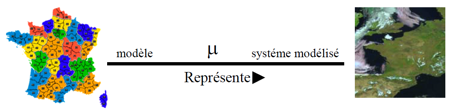
\includegraphics[width=1\textwidth]{images/Chapitre1/favresystememodele.png}
 \end{center}
 \caption{Relation entre système et modèle \protect\cite{favre2006ingenierie}}
 \label{fig:systemModele}
\end{figure}

Cette définition n'est pas restreinte à l'informatique et pourrait s'appliquer à 
n'importe quel système. 
La figure~\ref{fig:systemModele} reprend l'exemple connu de la cartographie où 
une carte géographique joue le rôle de modèle pour une région donnée jouant 
alors le rôle de système modélisé. 

L'intérêt de l'IDM est de produire des modèles exploitables informatiquement. 
Ceci n'est possible que si ces modèles sont décrits par des langages formels. Il 
devient alors important de bien définir ces langages à l'aide de métamodèles

\subsubsection{Métamodèle et ConformeÀ}
L'originalité de l'IDM ne réside pas dans la relation ReprésentationDe qui 
trouve plutôt son origine dans les méthodes de modélisation telles que Merise ou 
SSADM. L'apport de l'IDM est dans l'utilisation systématique de métamodèles pour 
la description des langages de modélisation. 

Il existe plusieurs définitions de la notion de métamodèle dans la littérature. 
Cependant la définition suivante est communément admise 
\cite{bezivin2004rapport}.

\begin{definition}
Un métamodèle est un modèle du langage de modélisation qui sert à exprimer les 
modèles.
\end{definition}
Une autre définition courante mais erronée de la notion de métamodèle suppose 
qu'un métamodèle est un modèle d'un modèle. La figure~\ref{fig:modelofmodel} 
reprend l'exemple de la cartographie évoquée plus haut. Nous appliquons 
récursivement la relation \textit{ReprésentationDe} $(\mu)$ au territoire 
français. Ici une carte de la France joue le rôle de modèle du territoire 
français et un fichier XML joue le rôle de modèle de la carte. Dans ce contre 
exemple, le fichier XML n'est pas un métamodèle de la France. Un métamodèle 
n'est donc pas un modèle d'un modèle.

\begin{figure}[!htbp]
 \begin{center}
  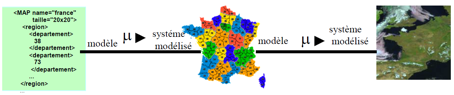
\includegraphics[width=1\textwidth]{images/Chapitre1/modelofmodel.png}
 \end{center}
 \caption{Modèle de modèle selon l'exemple de la cartographie 
\protect\cite{favre2006ingenierie}}
 \label{fig:modelofmodel}
\end{figure}

Par ailleurs, le concept de métamodèle induit la deuxième relation fondamentale 
de l'IDM liant un modèle à son métamodèle. Cette relation est nommée 
\textit{ConformeÀ} et notée $\chi$ \cite{bezivin2004search} 
\cite{favre2004towards}. La figure \ref{fig:carteFavre} reprend l'exemple de la 
cartographie où la légende de la carte joue le rôle de métamodèle ($\chi$) pour 
une carte de la France. En effet, pour être lisible, la carte doit être conforme 
à la légende.

\begin{figure}[!htbp]
 \begin{center}
  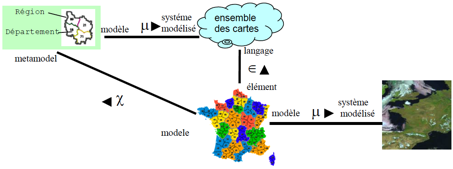
\includegraphics[width=1\textwidth]{images/Chapitre1/cartecompleteIDM.png}
 \end{center}
 \caption{Relations entre système, modèles, métamodèle et langage de 
modélisation \protect\cite{favre2006ingenierie}}
 \label{fig:carteFavre}
\end{figure}

\subsection{Transformation de modèle}
Dans la partie précédente, nous avons introduit les concepts fondamentaux de 
l'IDM que représentent la notion de modèle et la relation 
\textit{ReprésentationDe} ainsi que la notion de métamodèle et la relation 
\textit{ConformeÀ}. Comme expliqué, la préoccupation majeure de l'IDM est de 
rendre les modèles opérationnels sur tout le cycle de vie des systèmes 
logiciels, depuis l'analyse et la conception jusqu'à la maintenance et 
l'évolution. Ainsi, la transformation de modèle se retrouve au cœur de l'IDM car 
c'est à travers elle que se fait l'automatisation des traitements apportés aux 
modèles. Nous allons d'abord donner une définition de la notion de 
transformation de modèle puis en présenter les types et les usages.

\subsubsection{Définition de la transformation de modèle}
L'OMG définit une transformation de modèle comme «~le processus consistant à 
convertir un modèle en un autre modèle d'un même système~» \cite{omg2011meta}. 

\cite{kleppe2003mda} proposent une définition moins générique en insistant sur 
l'aspect automatique de ce processus, ainsi, «~une transformation de modèle 
consiste en la génération automatique d'un modèle source en un modèle cible, 
selon une description établie de cette transformation~». Cette définition 
implique aussi qu'une transformation est décrite à un plus haut niveau 
d'abstraction : au niveau d'un métamodèle auquel elle doit se conformer. 

\cite{mens2006taxonomy} étendent cette définition en considérant qu'une 
transformation est une opération qui peut avoir en entrée un ou plusieurs 
modèles source et en sortie un ou plusieurs modèles cible~: 

\begin{definition}
Une transformation génère automatiquement un ou plusieurs modèles cible à partir 
d'un ou plusieurs modèles source, selon une description établie de la 
transformation. 
\end{definition}

C'est cette dernière définition que nous allons adopter dans ce document. Par 
ailleurs, notons que, si les métamodèles source et cible sont différents, la 
transformation est dite exogène. Si les métamodèles source et cible 
correspondent au même métamodèle, la transformation est dite endogène. Ces 
termes ont été introduits par \cite{mens2006taxonomy}.

\subsubsection{Composants d'une transformation de modèle} 
La figure \ref{fig:composantTransfo} illustre les composants d'une 
transformation de modèle~:~les modèles source, les modèles cible, la définition 
de la transformation et le moteur qui va opérer la transformation selon sa 
définition. 

La description de la transformation spécifie comment un ou plusieurs modèles 
source sont transformés en un ou plusieurs modèles cible. Elle est écrite dans 
un langage de transformation de modèle. Par exemple, si c'est un langage à base 
de règles, la description de la transformation consiste en un ensemble de règles 
de transformation à opérer \cite{kleppe2003mda}. 

Un moteur de transformation exécute ou interprète la description. Il applique 
donc la description aux modèles source pour produire les modèles cible en 
suivant les étapes ci-dessous \cite{tratt2005model}~:

\begin{itemize}
\item Identifier l'élément du ou des modèles source à transformer.
\item Pour chaque élément identifié, produire l'élément cible qui lui est 
associé dans le ou les modèles cible.
\item Produire une trace de la transformation qui lie les éléments du ou des 
modèles cibles aux éléments du ou des modèles source.
\end{itemize}

\begin{figure}[!htbp]
 \begin{center}
   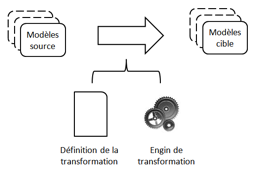
\includegraphics[width=0.7\textwidth]{images/Chapitre1/composanttransfo.png}
 \end{center}
 \caption{Composants d'une transformation de modèle}
 \label{fig:composantTransfo}
\end{figure}

\subsubsection{Usages de la transformation de modèles }
Les transformations de modèles sont au cœur d'une démarche dirigée par les 
modèles~:~elles permettent d'automatiser les manipulations subies par les 
modèles telles que la modification, la création, l'adaptation, la composition ou 
encore le filtrage de modèles, à travers la réutilisation systématique 
d'informations contenues dans les modèles existants. 

Il est possible de recourir aux transformations de modèles sur tout le cycle de 
vie d'un système. Les usages les plus répondus sont le raffinement, 
l'intégration d'outils, la composition, l'analyse, la simulation et 
l'optimisation que nous présentons dans la suite de ce document. 

\begin{description}

\item \textbf{Raffinement}

Le raffinement consiste à rajouter plus de détails au modèle initial. Ce type de 
transformation peut aussi bien être endogène (métamodèles source et cible 
identique) ou exogène (métamodèle source et cible différents). Le raffinement se 
prête parfaitement à toute la partie descendante du cycle en V où les modèles 
passent à des niveaux d'abstraction plus bas. Ceci revient à faire des 
transformations successives de type modèle-à-modèle et une transformation de 
type modèle-à-texte pour aboutir au code final.

Raffiner un modèle revient à décomposer des concepts de haut niveau, à choisir 
un algorithme particulier, à spécialiser un concept pour un contexte donné ou 
encore à le concrétiser sous forme d'une solution exécutable par une machine en 
générant le code à partir de modèles de plus haut niveau d'abstraction 
\cite{czarnecki2000intentional}. 

\item \textbf{Intégration d'outil}

Il existe une panoplie d'outils disponibles pour créer, manipuler, analyser ou 
encore simuler des modèles. Souvent ces outils utilisent des métamodèles 
internes et des espaces techniques qui leurs sont propres. Ainsi, l'échange de 
modèle entre ces outils est compromis et l'interopérabilité est fortement 
entravée. L'utilisateur se trouve obligé d'utiliser un seul et même outil sur 
tout le cycle de vie du système et ne peut donc pas tirer avantage des 
possibilités offertes par d'autres outils plus adaptés à ses besoins à certaines 
étapes.

L'intégration d'outil est une solution pour palier la divergence syntaxique et 
sémantique des outils et des langages de modélisation par le biais la 
transformation de modèle \cite{tratt2005model}. Ce type de transformation permet 
de naviguer entre deux métamodèles, de synchroniser des modèles qui évoluent 
séparément sur des outils distincts, de faire des mapping entre métamodèles pour 
maintenir la cohérence des modèles conformes à ces métamodèles. Il sera donc 
possible de faire appel à des outils mieux adaptés à chaque étape du cycle de 
vie.

\item \textbf{Composition}

Pour réduire la complexité inhérente à la modélisation et à l'analyse de grands 
systèmes, tels que les Smart Grids par exemple, il est possible d'adopter une 
approche par points de vue qui permet de séparer les préoccupations. Les modèles 
produits correspondent donc à ces différents points de vue qu'on peut ainsi 
valider séparément dans un premier temps. A l'issue de cette approche modulaire, 
on pourra composer ces modèles, c'est-à-dire les assembler, pour aboutir un 
modèle global du système.

Dans le cas le plus simple, les deux modèles à composer sont conformes à un même 
métamodèle. Cependant, il est aussi possible de composer deux modèles conformes 
à deux métamodèles différents. 

Les deux modèles à composer peuvent aussi présenter des concepts en commun. Deux 
techniques existent pour composer des modèles, que nous illustrons dans la 
figure \ref{fig:compoExemple}~:

\begin{itemize}
\item La première technique consiste à les fusionner. Dans ce cas, le modèle 
final résultant de la composition doit contenir toutes les informations issues 
des modèles initiaux, sans duplication des informations communes 
\cite{bezivin2006canonical}.
\cite{fleurey2008generic} présente un framework générique capable de composer 
des modèles indépendamment de leurs langages de modélisation. L'approche 
consiste à identifier les éléments qui représentent le même concept dans les 
deux modèles à composer et à les fusionner dans un nouveau modèle qui représente 
une vue intégrée de ces concepts. Il est aussi possible de spécialiser le 
framework pour un métamodèle particulier mais qui reste conforme au MOF.

\item La deuxième technique consiste à les tisser. Dans ce cas, on crée des 
correspondances entre les éléments qui représentent un même concept. Un 
métamodèle générique est créé pour définir les correspondances qui sont donc 
modélisées dans le modèle final. On y retrouve donc les éléments en commun 
dupliqués mais liés par un lien de correspondance. 
\end{itemize}

Il est à noter que le modèle issu du tissage de deux modèles $M_{A}$ et $M_{B}$ 
peut être utilisé comme modèle intermédiaire que l'on note $M_{T}$ pour la 
fusion de $M_{A}$ et $M_{B}$. Dans ce cas L'opération de fusion consiste à 
produire un modèle $M_{AB}$ en prenant comme entrée $M_{A}$, $M_{B}$ et $M_{T}$. 
Cette technique est notamment utilisée par \cite{del2007semi} pour la 
composition semi-automatique de modèles.

\begin{figure}[!htbp]
 \begin{center}
  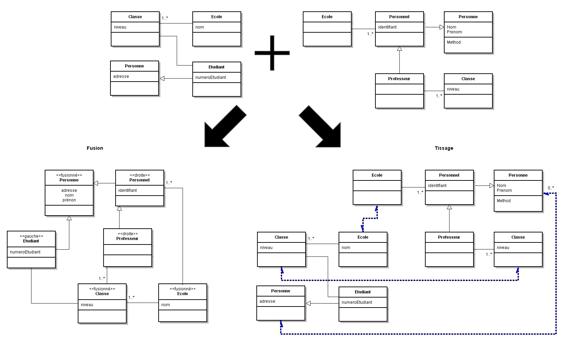
\includegraphics[width=1\textwidth]{images/Chapitre1/compoExemple.png}
 \end{center}
 \caption{Exemple de composition de deux modèles}
 \label{fig:compoExemple}
\end{figure}

\item \textbf{Simulation}

La transformation de modèle peut être utilisée pour simuler des modèles. En 
effet, une transformation de modèle peut mettre à jour le système modélisé. Dans 
ce cas, le modèle cible est une mise à jour du modèle source et la 
transformation est de type sur-place (modèles source et cible confondus). 

Par exemple, \cite{syriani2011multi} simule un comportement simple d'un jeu de 
Pacman en utilisant la transformation de modèle. La transformation spécifie les 
règles de transition qu'une instance du jeu peut prendre (Pacman et fantôme se 
trouvant dans la même case, Pacman et pomme se trouvant dans la même case, 
etc.). En ingénierie des langages, ceci revient à définir la sémantique 
opérationnelle d'un langage de modélisation. L'exécution de la transformation 
anime le modèle en fonction du comportement qu'on lui confère.

La transformation peut aussi être utilisée comme intermédiaire dans la 
simulation de modèle. Des modèles en entrée d'un outil de simulation externe 
sont produits par une transformation des modèles qu'on souhaite simuler. Cette 
technique permet de tirer profit d'outils de simulation existant sur le marché 
en utilisant l'intégration d'outils.

\item \textbf{Analyse et optimisation}

La transformation de modèle peut être utilisée pour les activités d'analyse de 
modèle. Une analyse simple telle que le calcul de métrique de similarité entre 
deux modèles via la transformation de modèle est donnée dans \cite{del2007semi} 
avec un modèle de transformation écrit en ATL \cite{jouault2006transforming}. 

Des analyses plus complexes sont possibles grâce à l'intégration d'outils 
d'analyse externes vers lesquels les modèles source sont transformés.

\cite{biehl2010integrating} propose d'utiliser la transformation de modèle pour 
l'analyse de sûreté de fonctionnement dans le domaine de l'automobile. Les 
modèles source sont transformés en modèles conformes au métamodèle de l'outil 
d'analyse de sûreté de fonctionnement retenu.
 
L'optimisation vise à améliorer les propriétés non fonctionnelles des modèles 
telle que l'évolutivité, la fiabilité, la modularité, etc. L'optimisation est 
typiquement utilisée sur les modèles d'architecture. Les transformations 
utilisées pour l'optimisation sont de types endogènes car on cherche à affiner 
la conception de modèles existants. La réingénierie est un exemple de 
transformation utilisée pour optimiser les modèles~:~on cherche à améliorer la 
maintenabilité, la lisibilité et l'évolutivité des modèles.

\end{description}

\subsubsection{Approches existantes pour la transformation de modèle}  
Le recours à la transformation de modèle est l'objet de recherches informatiques 
antérieures à l'apparition de l'approche IDM. Par exemple, les compilateurs 
utilisent la transformation pour passer du code source au fichier binaire 
\cite{aho1985compilers}. Ce type de transformation est restreint au domaine de 
la programmation informatique. La transformation de modèle embrasse un domaine 
plus large encore.

Nous trouvons dans la littérature plus d'une trentaine d'approches différentes 
de transformation de modèle \cite{syriani2011multi}. Czarnecki et Helsen 
proposent une classification de ces approches selon plusieurs critères tels que 
le paradigme retenu pour définir la transformation, la relation entre les 
modèles sources et cibles, la directivité de la transformation, le nombre de 
modèles cible et source, l'orchestration et l'ordonnancement des règles de 
transformation, etc. \cite{czarnecki2006feature}.

\cite{blanc2011mda} retient trois grandes catégories d'approches~:

\begin{itemize}
\item Par programmation

Les modèles offrent une interface qui permet d'écrire les transformations dans 
un langage de programmation. Mais cette technique relève plus de la 
programmation que de la modélisation. Ce sont en fait des applications 
informatiques qui ont la particularité de manipuler des modèles. L'avantage de 
cette approche est que l'on utilise un langage de programmation généraliste tel 
que Java ou C++ pour écrire les transformations. Ainsi le programmeur n'a pas 
besoin d'apprendre un nouveau langage. Cependant ces applications ont tendance à 
devenir difficilement maintenables. 

\item Par template 

Dans cette approche on définit des canevas des modèles cibles. Ces modèles 
contiennent des paramètres qui seront remplacés par les informations contenues 
dans les modèles source. Ce type de transformation est souvent utilisé pour les 
transformations modèle-à-texte et est associé au visitor-pattern qui va 
traverser la structure interne du modèle source. Cette approche est utilisée par 
l'outil Enterprise Architect par exemple. 

\item Par modélisation

Cette approche vise à appliquer les principes de l'IDM aux transformations de 
modèles elles-mêmes. Ainsi, on produit des modèles de transformation prennes, 
réutilisables et indépendants des plates-formes d'exécution 
\cite{bezivin2006model}. 

Pour cela, on utilise des langages de modélisation dédiés à l'activité de 
transformation de modèles. Cette approche considère donc la transformation comme 
un modèle à part entière conforme à un métamodèle de transformation. La figure 
\ref{fig:TransfoPrincipe} , illustre cette approche en positionnant la 
transformation sur les différents niveaux d'abstraction de l'IDM. Elle corrobore 
ainsi la vision unificatrice de l'IDM à travers le paradigme du « tout est 
modèle » \cite{bezivin2005unification}. Le langage de transformation ATL, que 
nous présentons dans la section~\ref{sec:ATL}, a été développé dans ce sens. 

\end{itemize}

\begin{figure}[!htbp]
 \begin{center}
  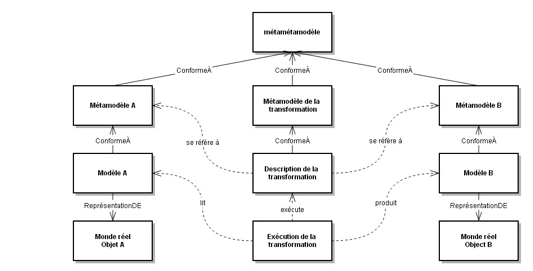
\includegraphics[width=1\textwidth]{images/Chapitre1/transfoPrincipe.png}
 \end{center}
 \caption{Méta niveaux d'une transformation de modèle}
 \label{fig:TransfoPrincipe}
\end{figure}

\subsection{Langages et outils pour la transformation de modèle}
Dans cette section, nous introduisons succinctement quelques langages et outils 
dédiés à la transformation de modèles, sans viser à l'exhaustivité.

\subsubsection{ATL}
\label{sec:ATL}
Atlas Transformation Language (ATL) \cite{jouault2006transforming} 
\cite{jouault2008atl} est né de la volonté de proposer des langages de 
modélisation dédiés à la transformation de modèle en définissant un métamodèle 
et des outils pour l'exécution des transformations. Il permet de réaliser des 
transformations de type modèle-à-modèle et de type modèle-à-texte.

ATL  est un langage hybride (déclaratif et impératif) à base de règles OCL (OMG 
2014). Une règle déclarative, appelée Matched rule, permet de décrire 
l'implémentation de mapping simples entre les modèles source et cible en 
utilisant des patrons source (\textit{InPattern}) mappés avec les éléments 
source et des patrons cibles (\textit{outPattern}) mappés avec les éléments 
cible. 

L'approche impérative explicite les étapes d'exécution de la transformation à 
travers les Helpers. Ce mécanisme de Helpers permet en outre d'éviter la 
redondance de code et la création de longues règles écrites en OCL, ce qui 
confère une meilleure lisibilité aux programmes ATL. 

Une transformation écrite en ATL est composée d'un ensemble de règles qui 
spécifient comment créer et initialiser les éléments des modèles cible. Il n'est 
pas possible de spécifier l'ordre d'exécution des règles de transformation. Cet 
ordre est établi automatiquement, exception faite pour les \textit{lazy rules} 
qui ont besoin qu'on fasse spécifiquement appel à elles. ATL est conforme au 
méta-métamodèle MOF et est doté d'une syntaxe concrète textuelle. Il est intégré 
à l'environnement Eclipse. Une transformation prend en entrée un ensemble de 
modèles conformes à Ecore (EMF 2014) ou KM3 \cite{jouault2006km3}.

ATL ne prend pas en charge les transformations incrémentales. Il commence par 
lire entièrement les modèles source et génère des modèles cible complet. Les 
modifications manuelles dans les modèles cible ne sont donc pas préservées si 
l'on opère une nouvelle transformation.

ATL peut réaliser des transformations sur  place, c'est-à-dire, une 
transformation où le modèle source et le modèle source sont confondus en 
utilisant le mode raffinement de modèle. Cependant ce mode présente quelques 
limitations avec certaines fonctionnalités comme celle des \textit{lazy rules}.

\subsubsection{QVT}
Le framework Query View Transformation (QVT) \cite{kurtev2008state} 
\cite{omg2011meta} a rejoint la batterie de standards de l'OMG. Le métamodèle de 
QVT est conforme au MOF. Comme ATL, QVT se base sur OCL pour accéder aux 
éléments des modèles.
QVT définit trois langages de transformation de type modèle-à-modèle. 
QVT-Relations (QVT-R) et QVT-Core (QVT-C) sont des langages déclaratifs qui 
adressent deux niveaux d'abstraction différents. QVT-Operational Mappings 
(QVT-OM) est un langage impératif qui étend QVT-R et QVT-C.

QVT-R est un langage de transformation de haut niveau d'abstraction doté de 
syntaxes concrètes textuelle et graphique. Les transformations, 
bidirectionnelles, sont spécifiées sous forme de relations entre les modèles 
source et cible. Une transformation a pour but de vérifier la cohérence entre 
deux modèles, renforcer la cohérence en modifiant le modèle cible, synchroniser 
deux modèles ou encore pour raffiner un modèle par une transformation sur-place. 
La sémantique de QVT-R est définie par une transformation vers QVT-C.

QVT-C est un langage de transformation de bas niveau qui sert de base pour 
QVT-R. Les deux ont le même niveau d'expressivité. Une transformation consiste 
en la déclaration de mapping entre les métamodèles source et cible en utilisant 
des patterns. Contrairement à QVT-R, la traçabilité est explicitement définie à 
travers les liens entre les métamodèles.

QVT-OM est un langage de transformation impératif qui étend QVT-R avec des 
constructions impératives basée sur une extension impérative de OCL. Les 
transformations sont unidirectionnelles mais établissent explicitement des 
modèles de traçabilité.

QVT est aussi doté d'un mécanisme de \textit{blackbox} qui permet de faire appel 
à des algorithmes complexes écrits dans n'importe quel langage de programmation 
et d'utiliser des librairies existantes. Mais ce mécanisme rend la 
transformation opaque puisqu'il n'est pas contrôlé par le moteur d'exécution. 
Nous pouvons citer SmartQVT ou encore ModelMorf comme machines d'exécution de 
transformation écrite en QVT.

\subsubsection{Kermeta}
Kermeta est un langage généraliste de méta-modélisation exécutable et de 
méta-programmation orientée objet qui peut aussi décrire des transformations de 
modèle. Intégré à EMF, il est doté d'un métamodèle conforme au MOF qu'il étend 
avec un langage d'action impératif utilisé pour écrire le corps des opérations 
définies sur les concepts d'une syntaxe abstraite (ce qui revient à doter une 
syntaxe abstraite d'une sémantique opérationnelle). On peut ainsi décrire 
n'importe quel traitement sur un modèle ce qui est assimilé à une transformation 
de modèle.

Le langage d'action de Kermeta permet d'écrire des expressions impératives qui 
spécifient explicitement la construction des éléments des modèles cible. A 
l'inverse de QVT-OM, Kermeta n'est pas un langage à base de règles.  
Kermeta est capable de gérer les exceptions mais les transformations 
multidirectionnelles ne sont pas supportées par les outils d'exécution. Il en 
est de même pour la transformation incrémentale. Les modèles source sont lus en 
une seule fois et les modèles cible sont produits complets lors de l'exécution 
de la transformation.




    %!TEX  root = main.tex
\chapter{Motivations et problématique}
\label{ch:problematique}

\PartialToc

\section{Contexte industriel}

Dans cette partie, nous introduisons le concept de Smart Grid avant d'exposer
les raisons de l'avènement de ce nouveau paradigme des réseaux électriques.


\subsection{Qu'est ce qu'un Smart Grid ?}

Le terme «~Smart Grid~» est une appellation générale désignant les technologies 
«~intelligentes~» qui «~augmentent~»\footnote{À la manière de «~l'augmentation 
de l'humain~» qui désigne l'amélioration technique des performances humaines, 
aussi bien physiques, intellectuelles qu'émotionnelles \cite{le2013humain}.} 
les réseaux électriques actuels en améliorant leurs performances. 

Cette «~augmentation~» peut servir différents objectifs dépendant des limites du 
système électrique existant, du cadre de régulation, ainsi que de 
l'orientation politique des états. Il existe autant de définitions du terme 
«~Smart Grid~» que d'objectifs motivant son implémentation. 

En Europe, les exigences de régulation et les volontés politiques des états 
membres en matière d'écologie favorisent l'intégration des énergies 
renouvelables et la participation active des consommateurs. Les Smart Grids 
européens sont donc synonymes de producteurs d'énergie renouvelables et de 
compteurs intelligents. Pour l'\gls{etp}, les Smart Grids sont ainsi «~des 
réseaux électriques qui intègrent de manière intelligente les comportements et 
les actions de tous les acteurs connectés — les producteurs, les consommateurs 
et ceux qui consomment et produisent en même temps — pour garantir une 
fourniture d'électricité efficiente, durable, économique et sûre.~» \cite{ETP}.

Les Smart Grids américains mettent, quant à eux, l'accent sur la modernisation 
des réseaux de transport d'énergie souvent très mal entretenus. Les États Unis 
doivent en effet faire face un nombre de coupures de courant qui ne cesse 
d'augmenter, passant de 76 pannes en 2007 à plus de 300 en 2011 \cite{detroit}. 
Ces pannes sont aussi fréquentes qu'importantes. En 2003, un \textit{blackout} 
dans l'Ohio prive 50 millions de personnes d'électricité et coûte 6 milliards 
de dollars \cite{andersson2005causes}. Ces coupures sont dues à la combinaison 
de trois facteurs \cite{outages}:

\begin{itemize}
    \item une infrastructure électrique vieillissante, en grande partie
    mécanisée et souffrant du manque d'investissement~;
    \item une forte croissance démographique~;
    \item des conditions climatiques de plus en plus extrêmes.
\end{itemize}

Aux États Unis, moderniser le réseau électrique en investissant dans les Smart 
Grids est ainsi essentiellement guidé par un impératif de fiabilité. Pour 
définir les Smart Grids, le département de l'énergie américain (\textit{United 
States Department of Energy}) dresse une liste d'exigences mettant en avant la 
sûreté des réseaux électriques \cite{USDE}. Selon cette définition, un Smart Grid 
doit ainsi répondre aux exigences suivantes~:

\begin{itemize}
    \item auto-réparation en cas d'événements perturbateurs~;
    \item permettre la participation active des consommateurs~; 
    \item résilience face aux attaques physiques et cybernétiques~;
    \item fournir une électricité de qualité face aux besoins du 21\up{ème}
          siècle~;
    \item intégration de moyens de production et de stockage d'électricité~;
    \item exploitation optimisée des infrastructures et conduite efficace des 
réseaux électriques.
\end{itemize} 

À partir de ces deux définitions, nous constatons que l'obsolescence du système 
électrique (dans le cas des États Unis) et les impératifs régulatoires et 
écologiques (dans le cas de l'Europe) font de la mise à niveau des réseaux 
électriques un enjeu crucial. Cette mise à niveau passe d'abord par le 
déploiement des \gls{tic} et donc par l'implémentation des Smart Grids, plutôt 
que par le remplacement massif des infrastructures électriques existantes. 

Envisager uniquement le renforcement et de remplacement massif des 
infrastructures électriques du  réseau 
n'est en effet pas une solution optimale et semble difficilement réalisable 
compte tenu de la croissance démographique constante des zones urbaines et du 
coût important des investissements à consentir \cite{cre}.

\subsection{Contexte économique, cadre législatif et\\
modes de consommation en constante mutation}

Le système électrique actuel est mis à l'épreuve par l'entrée en jeu de nouveaux 
acteurs économiques et de nouveaux cadres législatifs. 

D'une part, la libéralisation du marché de l'électricité permet à un producteur 
quelconque de produire et de vendre son électricité après s'être convenablement 
raccordé au réseau électrique de distribution ou de transport (donc entre les 
centrales de production et les consommateurs). Contrairement aux centrales de 
production localisées en amont du réseau électrique de transport, ces sources 
d'énergie sont dites distribuées. Les sources d'énergie distribuées perturbent 
fortement la stabilité des réseaux électriques. En injectant du courant, elles 
peuvent déséquilibrer le niveau de tension du réseau, endommageant ainsi les 
équipements du système électrique tels que les transformateurs, les lignes et 
les protections. 

D'autre part, les enjeux environnementaux encouragent le recours aux énergies 
renouvelables. Dans sa directive du 23 avril 2009, la commission européenne fixe 
à 20\% la part de contribution des ressources renouvelables dans la production 
totale d'énergie à l'horizon de 2020. Les réseaux électriques sont de ce fait 
amenés à connaître une croissance constante de ces producteurs décentralisés 
dans les années à venir.

Cette même directive fixe à 20\% la réduction des émissions de gaz à effet de 
serre par rapport à leur niveau en 1990 et à 20\% l'augmentation de l'efficacité 
énergétique. Or les pics de consommation en période de pointe sont coûteux et 
émetteurs de CO\textsubscript{2}. Ces pics apparaissent typiquement en fin de journée d'un 
jour de semaine lorsque les gens allument leurs télévisions, plaques électriques 
et autres outils électroménagers en rentrant chez eux.  En effet, pour maintenir 
l'équilibre entre l'offre et la demande d'électricité en cas de pics de 
consommation, les producteurs recourent à des centrales à charbon, à fioul et à 
gaz comme l'illustre la figure~\ref{fig:courbeCharge}.


\begin{figure}[!ht]
 \begin{center}
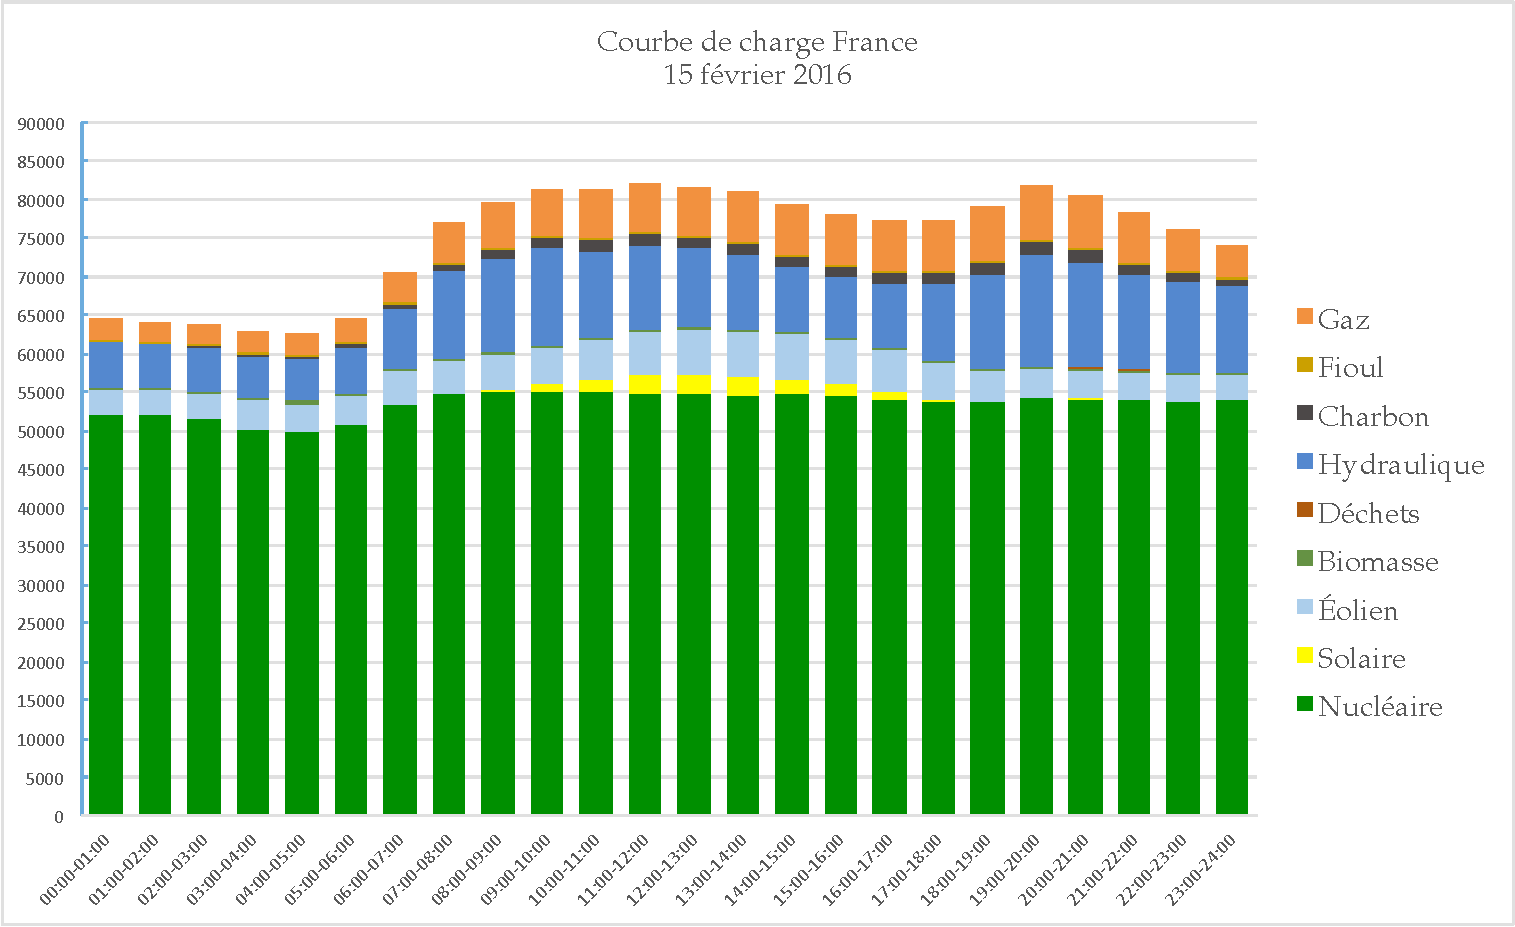
\includegraphics[width=1\textwidth]{figures/1_problematique/courbe_charge.pdf}
 \end{center}
 \caption{Placement du type d'énergie sollicitée sur la courbe de charge 
française du lundi 15 février 2016 (source RTE\protect\footnote{ Réseau Transport France (http://www.rte-france.com/)})}
 \label{fig:courbeCharge}
\end{figure}

Ces pics s'intensifient significativement avec l'émergence de nouveaux usages de 
consommation d'énergie dont, notamment, la mobilité électrique. En France, les 
pouvoirs publics estiment à deux millions le nombre de véhicules électriques en 
circulation en 2020. L'impact de ces véhicules sur l'équilibre entre l'offre et 
la demande n'est pas négligeable. En effet, la recharge complète d'un véhicule 
électrique ayant 150 km d'autonomie est équivalente en termes d'appel de 
puissance à~:
\begin{itemize}[noitemsep]
    \item un chauffe-eau si la recharge s'effectue en 8~h (recharge normale)~;
    \item un immeuble si la recharge s'effectue en 1~h (recharge accélérée)~;
    \item un quartier urbain si la recharge s'effectue en 3~min (recharge rapide).
\end{itemize}



\subsection{Architecture des Smart Grids : \\
vers des réseaux électriques flexibles et communicants}

Pour faire face aux mutations du contexte énergétique, les gestionnaires de 
réseaux électriques ne peuvent plus compter uniquement sur la conduite 
prévisionnelle du réseau électrique (peu réactive face à l'intermittence des 
énergies renouvelables par exemple) ni envisager le redimensionnement du réseau 
(onéreux et non optimal). 

La solution réside dans l'automatisation de la conduite des réseaux électriques, 
grâce a l'acquisition et l'exploitation en temps réel d'informations sur l'état 
des réseaux. Cela passe par le déploiement d'un réseau informatique au niveau 
des infrastructures électriques, et la mise en place dans le \gls{si} d'outils 
pour l'exploiter.

Ainsi équipés, les réseaux électriques s'apparentent à une toile d'araignée où 
les mailles interagissent constamment via des liens de communication. Ces 
mailles correspondent aux acteurs du système électrique~: consommateurs, 
producteurs ou les deux à la fois. Outre l'électricité, ces acteurs produisent 
et consomment de l'information en temps réel grâce aux modules logiciels dont 
ils sont équipés et à divers moyens de télécommunication, tels que les réseaux 
mobiles ou le \gls{cpl}. Ce partage permanent et 
instantané d'informations entre les équipements préserve la stabilité du 
système électrique tout en augmentant son efficacité énergétique.

Pour illustrer les possibilités offertes par les \gls{tic}, prenons l'exemple 
du pic de consommation de la fin de journée d'un jour en semaine. Grâce aux 
\gls{tic}, il devient possible d'agir sur la demande plutôt que sur l'offre. Le
distributeur d'électricité, s'appuyant sur des points de contrôle distants et 
des compteurs intelligents installés chez les clients pour envoyer et recevoir 
des informations et des consignes, peut alors adresser des demandes 
d'effacement aux consommateurs moyennant des incitations tarifaires. Il peut 
s'agir d'une coupure du chauffage pendant 15~min à 30~min d'un foyer ou d'un 
bureau bien isolé. Sans incidence sur le confort des consommateurs, ces 
demandes d'effacement aident à lisser la courbe de charge aux heures de pointe 
tout en évitant de mobiliser des centrales de production. 

Nés de la convergence des réseaux électriques et des \gls{tic}, les Smart Grids 
se composent de trois couches que nous retrouvons dans la figure~\ref{fig:archismartGrids}~:

\begin{enumerate}
    \item le premier niveau correspond à l'infrastructure et aux équipements 
    électriques acheminant l'électricité tels que les lignes et les 
    transformateurs~; 
    \item le second niveau correspond à l'infrastructure de communication 
    composée de différentes technologies de télécommunication comme la fibre 
    optique, le \gls{cpl}, ou encore la \gls{3g}~; 
    \item le troisième niveau correspond aux applications informatiques qui 
    incarnent «~l'intelligence~» du réseau. En utilisant des informations 
    délivrées en temps réel, ces applications calculent des consignes à envoyer 
    aux équipements concernés et automatisent ainsi la conduite du système 
    électrique.  Cette intelligence est centralisée au niveau des centres de 
    conduite du réseau ou distribuée sur les équipements électriques. 
\end{enumerate}

\begin{figure}[!htbp]
  
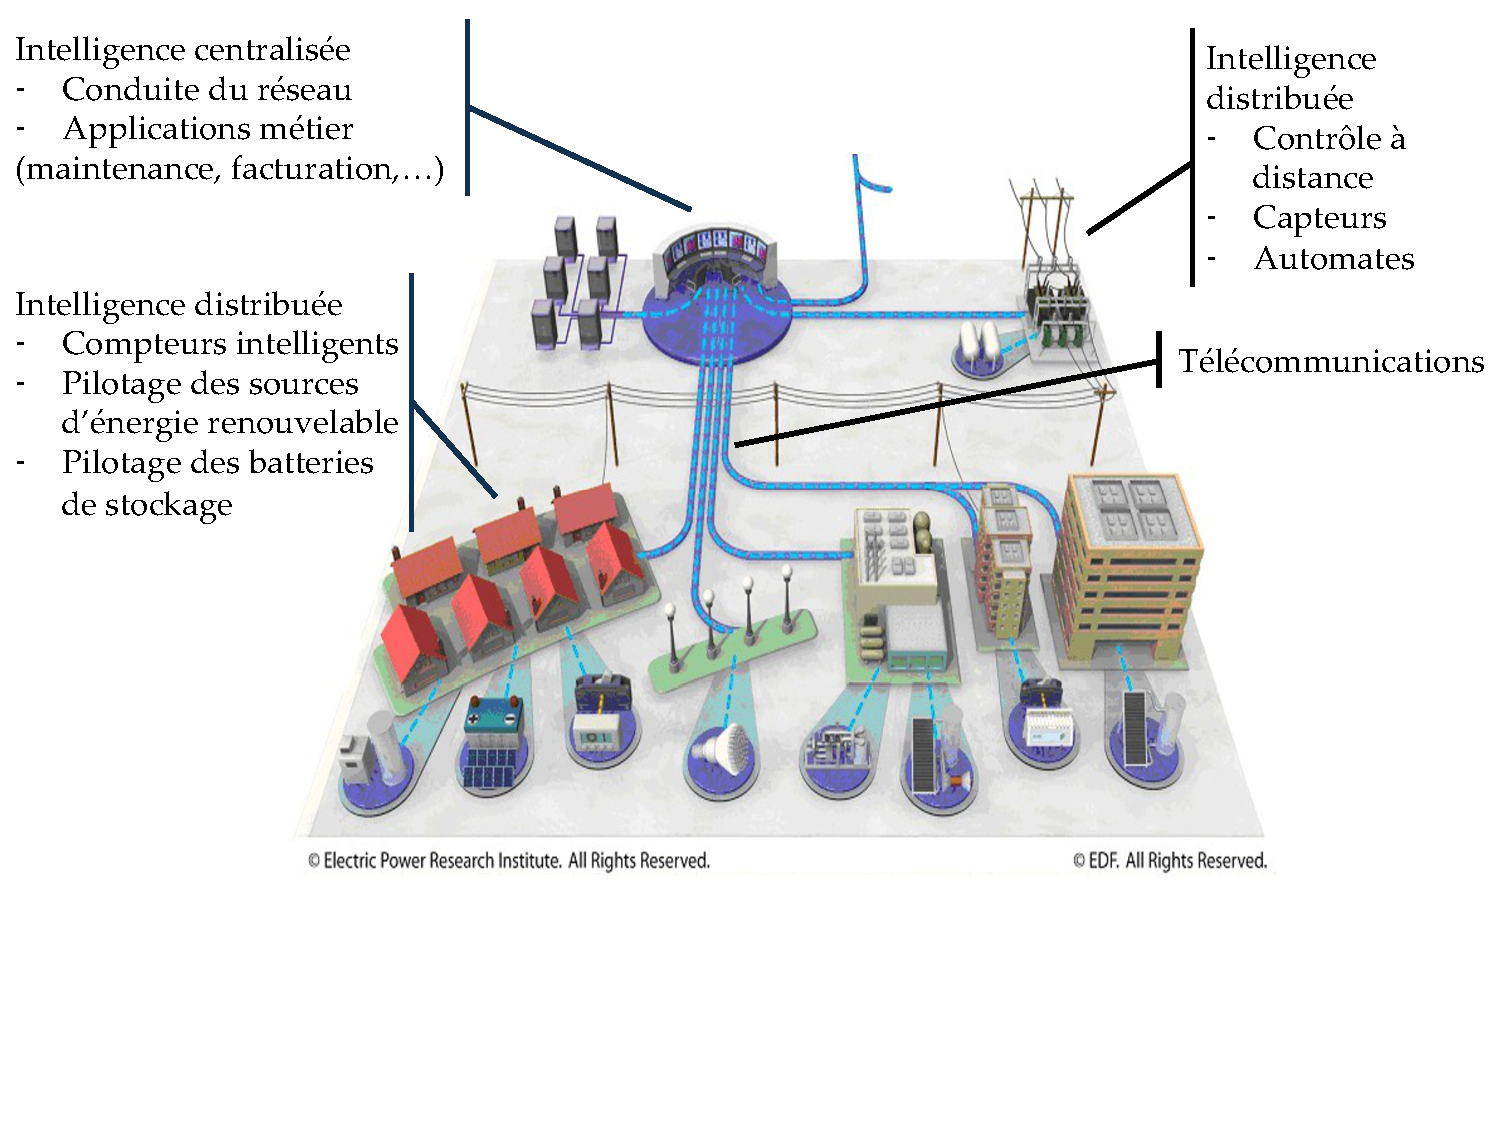
\includegraphics[trim= 0cm 4cm 0cm 0cm, width=1\textwidth]{figures/1_problematique/archiSmartGrids.pdf}
 \caption{Architecture des Smart Grids \protect\cite{favre2006ingenierie}}
 \label{fig:archismartGrids}
\end{figure}


%En effet, la libéralisation du marché de l'électricité exige que le 
%consommateur ait une connaissance en temps réel de l'évolution tarifaire 
%horaire 
%de l'électricité et qu'il puisse même choisir d'injecter sa propre propre 
%production d'énergie sur le réseau.

\section{Problématique industrielle}
%la nécessaire évolution des Systèmes d'Information pour la mise en œuvre d'une stratégie orientée Smart Grids

%Un Smart Grid est un réseau électrique intelligent permettant d'optimiser la 
%production, la distribution et la consommation d'électricité grâce à 
%l'introduction des Technologies de l'Information et de la Communication (TIC) 
%sur le réseau électrique \footnote{www.smartGrids-cre.fr}.

En traitant les données envoyées en temps réel par les capteurs installés sur 
les équipements électriques et chez les consommateurs, les \gls{si} calculent 
des consignes destinées à des organes télécommandés permettant ainsi de piloter 
les 
réseaux électriques à distance. 
Cette automatisation de la gestion des réseaux est une solution pour les adapter 
rapidement face aux contraintes qu'introduit l'intégration des énergies 
renouvelables et des nouveaux usages \cite{cre}. Les \gls{si} sont donc au cœur 
des 
enjeux Smart Grids.  

L'implémentation des Smart Grids va ainsi de pair avec la mise à niveau des 
\gls{si} des gestionnaires du réseau électrique. En effet, ces \gls{si} doivent 
pleinement intégrer les évolutions qu'induisent les Smart Grids au niveau des 
processus 
métier du gestionnaire de réseau, des acteurs impactés, des informations 
échangées ainsi que des applications informatiques et des infrastructures 
techniques sous-jacentes. Parmi ces évolutions nous citons~:

\begin{itemize}
    \item les nouveaux flux d'information provenant du réseau électrique~;

    \item l'entrée en jeu de nouveaux acteurs tels que les producteurs
    décentralisés (éolien, photovoltaïque)~;

    \item les nouveaux équipements communicants comme le compteur Linky 
(\gls{erdf} 
    annonce le déploiement de 30 millions de compteurs d'ici 
    2020\footnote{www.erdf.fr/Linky})~;

    \item les nouvelles réglementations et directives européennes (dans le cas 
    des gestionnaires de réseaux européens)~;

    \item les nouveaux usages comme les véhicules électriques ou encore les 
    maisons connectées.
\end{itemize}

Outre leurs \gls{si}, les gestionnaires de réseaux électriques doivent faire 
évoluer 
leurs stratégies de développement en envisageant de nouveaux modèles métier et 
de nouveaux partenaires, tout en tenant compte de l'émergence des nouvelles 
technologies et des exigences du législateur. Une étude américaine, menée par 
IBM, CISCO, EPRI et South Carolina Edison, fait état de cinq thèmes stratégiques 
clés pour l'implémentation des Smart Grids~:

\begin{itemize}

    \item \textbf{permettre au consommateur de contrôler sa consommation 
    d'énergie} et de réduire son empreinte carbone en utilisant des équipements 
    intelligents et des véhicules électriques et en produisant de l'énergie 
    renouvelable à domicile~;

    \item \textbf{améliorer la sécurité et la productivité des employés} en 
    mettant par exemple à leur disposition des outils performants pour le 
    contrôle à distance, des équipements de protection, et des applications 
    mobiles~; 

    \item \textbf{intégrer des sources d'énergie renouvelables} distribuées sur 
    le réseau en assurant la protection des équipements électriques, le 
    stockage de l'énergie et la stabilité du réseau~; 

    \item \textbf{améliorer l'efficience et la résilience du réseau} à travers 
    les systèmes de mesure en temps réel, l'analyse et le contrôle à distance~;

    \item \textbf{fournir les informations et la connectivité nécessaires} en
    developpant une infrastructure \gls{tic} pour répondre aux besoins 
    d'informatisation du réseau électrique. Ce dernier point est une condition 
    \textit{sine qua non} de la réalisation des quatre précédents.
\end{itemize}

Compte tenu de ces thèmes clés, les gestionnaires de réseaux envisagent des 
stratégies impliquant l'adoption de technologies Smart Grids. 
La mise en œuvre effective de ces stratégies demande l'automatisation des 
actions sur le réseau et du traitement des données, ce qui entraine donc le 
déploiement de nouveaux \gls{si}. Afin d'appréhender ces paradigmes naissants, 
des 
scénarios métier sont élaborés mais il est indispensable de les éprouver et de 
les valider avant d'envisager leur implémentation finale.

Plusieurs démonstrateurs physiques ont été déployés sur le terrain 
\footnote{www.erdf.fr/Carte\_demonstrateurs\_Smart\_Grids}. Ces projets pilotes 
permettent de mener des expérimentations en conditions réelles pour tester des 
fonctions et des services, comme par exemple le démonstrateur InfiniDrive 
\footnote{avem.fr/actualite-erdf-et-le-groupe-la-poste-lancent-le-projet-infini-drive-a-nice-3450.html} 
pour le pilotage des infrastructures de recharge de véhicules électriques ou le 
démonstrateur Venteea \footnote{www.venteea.fr} pour l'intégration d'une forte 
capacité éolienne dans un réseau rural. Cependant, les démonstrateurs 
nécessitent que le gestionnaire de réseau de distribution recrute des clients 
industriels et/ou domestiques qui acceptent d'avoir du matériel à tester chez 
eux. De plus, leur exploitation reste limitée par les réglementations en cours. 
Enfin, leur mise en place se révèle souvent longue et coûteuse. 

En plus de ces démonstrateurs, des réseaux de distribution d'expérimentation 
grandeur nature tel que Concept Grid \footnote{chercheurs.edf.com}, implanté à 
\gls{edf} Lab, permettent de tester les nouveaux équipements avant leur 
installation sur les réseaux du distributeur \gls{erdf}. Ces réseaux ont 
l'avantage de permettre la conduite de \textit{stress tests} en conditions perturbées, 
impossibles à réaliser dans le cadre de démonstrateurs, ceux-ci impliquant de 
vrais clients. Cependant, la taille réduite de ces réseaux reste limitante. 

Pour pallier toutes ces limitations, une troisième voie est la simulation. La 
simulation intègre les trois couches qui composent les Smart Grids~: 
l'infrastructure électrique (transformateurs, lignes, charges, sources), 
l'infrastructure de télécommunication (réseaux mobiles, \gls{cpl}) et enfin les 
\gls{si} qui 
les pilotent. Des simulateurs spécialisés dans la simulation de réseaux 
électriques (EMTP-RV, Dymola, PowerFactory, Eurostag, etc.) ainsi que des 
simulateurs de réseaux de télécommunication (OPNET, NS-3, OMNeT ++, etc.) ont 
déjà validé l'apport de la simulation dans leurs domaines respectifs. Toutefois, 
les \gls{si} sont souvent relégués à de simples modèles de calcul de consignes 
souvent 
développés en Matlab ou en C++ \cite{palensky2014simulating}. 

Dans ce contexte, la problématique industrielle dans laquelle  s'inscrivent nos 
travaux de recherche est donc la suivante~: 

\textbf{Comment valider une stratégie de développement orientée Smart Grids à 
travers la simulation de sa déclinaison au niveau du SI du gestionnaire du 
réseau électrique~?}

 
\section{Problématique de recherche}

%\subsection{Le recours à l'Architecture d'Entreprise}

Les technologies Smart Grids illustrent le défi que représente l'évolution des 
\gls{tic} et l'intégration des énergies renouvelables pour les gestionnaires de 
réseaux électriques. Jeremy Rifkin annonce même «~une troisième révolution 
industrielle, fondée sur le couplage des technologies de l’Internet et des 
énergies nouvelles~» \cite{rifkin2012troisieme}. 

Mais à l'ère numérique, l'adaptation au changement relève des préoccupations de 
toute entreprise s'appuyant sur les \gls{tic} pour mener ses 
activités. Le très haut niveau de concurrence que connait le secteur des 
technologies de l'information stimule l'innovation. Or ces technologies sont de 
plus en plus le moteur qui fait progresser les  métiers de l'entreprise. Être 
capable de s'adapter continuellement à l'évolution rapide et 
constante des \gls{tic} représente donc un véritable challenge pour les 
entreprises 
d'aujourd'hui.

Pour mener à bien tout changement, il est primordial de commencer par une 
description représentative de «~l'objet~» à changer, qu'il s'agisse d'une 
nouvelle version d'un avion, d'une voiture, d'un ordinateur ou encore d'une 
entreprise \cite{zachman1997enterprise}. Cette description représentative 
revient à concevoir l'architecture de l'objet en question. L'architecture en 
tant qu'activité est centrale dans plusieurs disciplines, allant de 
l'architecture du bâtiment à l'architecture logicielle, en ce qu'elle est un 
outil indispensable à la construction d'artefacts respectant les qualités 
attendues de l'objet final. En précurseur, Zachman \cite{zachman1997enterprise} 
recommande d'appliquer les principes d'architecture à l'entreprise pour faire 
face aux changements dictés par l'innovation technologique.

Les \gls{si} sont en première ligne dès qu'il s'agit de l'évolution des 
\gls{tic}. Nos 
travaux se sont donc d'abord portés sur l'évaluation de l'impact de cette 
évolution sur les \gls{si} de l'entreprise. De ce fait, nous nous sommes d'abord 
appliqués à décrire l'architecture de ces \gls{si} \cite{seghiri2015simulation}. 

Les changements apportés par ces technologies impactent cependant, non seulement 
les \gls{si}, mais l'entreprise dans son ensemble~: de sa stratégie à ses 
partenaires, en passant par ses objectifs, ses clients et ses processus métier. 
Par exemple, 
l'utilisation des véhicules électriques fait évoluer le \gls{si} du 
gestionnaire du réseau électrique qui doit mettre en place de nouvelles 
applications capables de bien gérer leur recharge. Mais il doit aussi faire 
évoluer son modèle métier en mettant à disposition de nouveaux contrats 
client favorisant la recharge hors de la période des pics de consommation par exemple, 
ou encore créer de nouveaux partenariats avec les constructeurs 
automobiles comme dans le cas d'\gls{edf} et Renault-Nissan qui collaborent sur 
un système de recharge pour véhicule électrique permettant à ce dernier de 
communiquer avec les bornes de recharge.

Évaluer l'adoption de nouvelles technologies de l'information oblige à prendre 
en compte l'entreprise dans son ensemble afin de garantir une cohérence entre 
la stratégie d'évolution adoptée et les \gls{si} qui implémentent cette 
stratégie. Parce que l'alignement entre la stratégie métier et le \gls{si} est 
au cœur de l'\gls{ea}\footnote{L'acronyme EA (\textit{Enterprise Architecture}) 
est souvent utilisé même dans la communauté francophone.} 
\cite{zachman1997enterprise}, nous
adoptons l'\gls{ea} pour évaluer l'impact des technologies Smart Grids sur les
gestionnaires des réseaux électriques. Il est en effet indispensable de
concevoir une architecture cible pour avoir  «~une vision générale de comment
une entreprise va mettre en œuvre sa stratégie~» \cite{ross2006enterprise}.

L'\gls{ea} participe à l'alignement des composants d'une entreprise en offrant 
une vision globale et transverse \cite{zachman1987framework}. Dans le contexte 
des 
Smart Grids par exemple, elle permet d'aligner efficacement les intérêts des 
acteurs impliqués dans leur implémentation tels que les experts métier, les 
conseillers stratégiques, les experts environnementaux ou encore les experts en 
normalisation.

L'exécution effective d'une stratégie est cependant confrontée à des barrières 
de communication au sein de l'entreprise \cite{vcater2010factors}. Le recours à 
l'\gls{ea} est d'autant plus justifié qu'elle représente un outil pour la 
transmission des objectifs stratégiques à tous les niveaux hiérarchiques de 
l'organisation en 
question \cite{kappelman2008enterprise}. 

Pour toutes ces raisons, nous souhaitons mettre à profit les principes 
d'\gls{ea} pour évaluer l'impact de l'adoption des technologies Smart Grids sur 
les \gls{si} des 
gestionnaires de réseaux électriques, tout en garantissant la cohérence entre la 
stratégie adoptée et les \gls{si} qui les implémentent. 

%\cite{buckl2010conceptual}. Le recours à l'architecture d'entreprise est ainsi 
%pleinement justifié.

%\subsection{Le recours à la simulation}

Les Smart Grids correspondent à des systèmes dynamiques et complexes 
\cite{monti_power_2010} étant donné le grand nombre de parties prenantes qui 
interagissent eux (tels que les producteurs d'énergie renouvelable ou les 
consommateurs actifs sur le réseau), tout en ayant des comportements autonomes 
et des objectifs différents. Les \gls{si} pilotant les  Smart Grids 
correspondent par conséquent à des systèmes dynamiques aux comportements 
complexes. Borshchev et 
Filippov\cite{borshchev2004system} affirment que le seul moyen d'adresser cette 
complexité est de simuler ces systèmes. La simulation est une technique connue 
pour valider ou critiquer la conception d'un système dès les premières étapes 
de son cycle de développement. Les acteurs impliqués dans le déploiement des 
Smart Grids acquièrent, par la  simulation, une connaissance approfondie et 
directe des modèles créés pour valider ou critiquer leur choix d'implémentation.

Néanmoins, les approches d'\gls{ea} se focalisent le plus souvent sur des 
aspects statiques et structurels tels que les interconnexions entre les 
différentes applications métier \cite{buckl2008towards}. De plus, les modèles 
issus de ces 
approches sont ne sont pas exécutables et sont conçus en 
priorité pour la documentation et la communication entre parties prenantes 
\cite{kulkarni2013modelling}. Notre problématique de recherche se résume de ce 
fait dans la question suivante :

\vspace*{1em}
\begin{framed}
{\bfseries Quels méthodes, modèles et outils adopter pour simuler une 
architecture d'entreprise afin de la valider?}
\end{framed}





    \chapter{Architecture d'Entreprise}
\label{chap:EA}

\section{Notions de bases de l'Architecture d'Entreprise}

Comme expliqué dans notre problématique de recherche (ajouter cf problématique de recherche),   nos travaux se sont d'abord portés sur la modélisation et la simulation des SI en prenant les Smart Grids comme cas d'application. Cependant le SI n'est pas indépendant de la réalité de l'entreprise. Notre approche doit de ce fait prendre en compte la stratégie de l'entreprise et ses objectifs métier. Nous souhaitons garantir une cohérence et une traçabilité entre les impératifs de l'entreprise et son SI. Il est en effet indispensable de s'assurer de l'alignement entre le métier et le SI de l'entreprise avant toute simulation. 

L'alignement métier/SI est au cœur de l'Architecture d'Entreprise. Les applications informatiques ne cessent de se démultiplier et prennent une place des plus en plus prééminente dans le fonctionnement des entreprises. Le besoin d'avoir une vision globale de l'entreprise et de son SI donne ainsi naissance à l'Architecture d'Entreprise, une discipline à part entière qui traite le SI en le corrélant au reste de l'entreprise. 

C'est pour cette raison que nous consacrons cette partie de l'état de l'art à l'Architecture d'Entreprise. Nous commençons par définir les termes de SI et d'Architecture d'Entreprise. 
  
\subsection{Terminologie}

\textbf{Système d'Information}

Selon Robert Reix, le SI est «~un ensemble organisé de ressources : matériel, 
logiciel, personnel, données, procédures permettant d'acquérir, de traiter, de 
stocker des informations (sous forme de donnée, textes, images, sons, etc.) dans 
et entre des organisations.~»

Nous adoptons cette définition car elle a l'avantage de ne pas réduire le SI 
d'une organisation à son système informatique. Le système informatique est constitué de 
l'ensemble du patrimoine matériel (hardware) et applicatif (software) de la dite 
organisation et a pour objectif d'automatiser le traitement de l'information. 
Nous adoptons l'acronyme IT (\textit{Information Technologies}) pour le 
différencier du SI.

On suppose souvent que les SI sont totalement informatisés et c'est une des 
raisons qui mènent à confondre SI et et IT. Cependant, le SI comprend non seulement 
le système informatique mais aussi des ressources humaines tels que les partenaires 
ou le personnel et ides ressources mmatérielles comme les procédures de gestion ou le savoir-faire métier.

\textbf{Architecture d'Entreprise}

Selon Zachman, l'Architecture d'Entreprise est «~un ensemble pertinent d'artefacts de conception ou de représentations descriptives pour décrire une entreprise de manière à ce cette entreprise soit créée en respectant certaines exigences et à ce qu'elle soit facilement maintenue le long de son cycle de vie~» \cite{zachman1997enterprise}. 

Zachman voit ainsi dans l'architecture un gage de qualité et de maintenabilité. L'architecture d'entreprise revient à appliquer à l'entreprise les principes de de l'architecture telle. qu'elle est pratiquée dans de nombreuses disciplines comme l'architecture du bâtiment. En effet, construire une maison en procédant chambre par chambre sans plan d'architecture général peut mener à un résultat peu probant. De même, le développement d'une organisation, sans 
architecture de référence globale et préalable, risque de mener à une 
duplication de ses ressources et altère par conséquent son efficacité, sa cohérence interne ainsi que toute volonté de changement \cite{zachman1997enterprise} \cite{bernard2012introduction}. 

Il est important de noter que le terme architecture d'entreprise peut prêter à 
confusion car il est à la fois utilisé pour désigner (1) l'activité de 
conception d'une architecture i.e. la description des éléments composant 
l'organisation en question et leurs relations mais aussi (2) l'ensemble des 
artefacts résultant de cette activité. 
Pour éviter toute confusion, nous désignons l'activité de conception par le 
terme architecture d'entreprise et résultat de cette activité comme étant 
l'architecture de l'entreprise.

%S'agissant du terme «~entrerprise~», Scott Bernard \cite{bernard2012introduction} y réfère comme une organisation ou une sous-partie d'une organisation qui poursuit des objectifs 
%communs, en s'appuyant sur les mêmes processus et en utilisant les mêmes 
%ressources. Une entreprise peut être publique ou privée, avoir ou pas un but lucratif. 

\subsection{Évolution de l'Architecture d'Entreprise}

L'architecture d'entreprise est ancrée dans l'architecture de systèmes 
informatique \cite{kappelman2008enterprise}. Elle a ensuite évolué vers une 
architecture qui comprends l'IT mais aussi certains aspects métier de l'entreprise 
\cite{winter2006essential}  jusqu'à adresser l'ensemble de l'entreprise en 
intégrant la stratégie de l'entreprise et ses processus décisionnels 
\cite{ross2006enterprise} allant même jusqu'à aborder l'environnement dans 
lequel elle évolue.

En effet, l'origine de l'EA\footnote{D'après Scott Bernard 
\cite{bernard2012introduction}, le terme Architecture d'Entreprise a fait sa 
première apparition dans le livre de Steven Spewak intitulé «~Enterprise 
Archietcture Planning~:~developing a blueprint for data, applications and 
technology~» \cite{spewak1993enterprise}.} remonte au travaux de Zachman, souvent 
considérés comme précurseurs. Il y propose un cadre d'architecture pour l'IT 
\cite{zachman1987framework}.

L'Architecture d'Entreprise (AE) a donc été initialement  conçue pour 
optimiser la gestion du patrimoine applicatif et de l'infrastructure technique d'une  
entreprise. À ses débuts, l'AE se focalise sur des artefacts purement IT (data, logiciels, équipements) pour 
rationaliser les l'utilisation des ressources informatiques 
\cite{winter2006essential} tout en répondant aux besoins métier de l'entreprise. 
L'AE est alors guidée par les pratiques d'ingénierie logicielle. 

 

Cependant, le rôle de plus en plus prégnants de l'IT et son impact sur le 
c\oe{}ur de métier des organisations ainsi que l'accroissement de sa complexité 
\cite{ranganathan2005enterprise} ont fait de l'architecture de l'IT d'une 
entreprise une problématique inhérente à l'architecture de l'ensemble de 
l'entreprise. Ainsi, l'AE a commencé à intégrer des aspects métier tels que les 
objectifs de l'organisation, les processus métier, les indicateurs de 
performances \cite{winter2006essential}. En intégrant ainsi des problématiques 
métier, L'AE ne relève plus de l'architecture IT mais de l'architecture du SI 
dans son ensemble.

Pour Scott Bernard, l'AE doit même aller plus loin en intégrant la stratégie de 
l'entreprise \cite{bernard2012introduction} dans son champs de discipline pour 
profiter pleinement de l'ensemble des ressources de l'entreprise (métier, IT, 
humaines, etc.). Ainsi, le terme "~entreprise~" implique une vue stratégique de 
haut niveau de l'organisation dans son ensemble. Quand au terme 
"~architecture~", il sous-entend la mise en place d'un cadre structuré pour 
l'analyse, le planning, et le développement de toutes les ressources dont 
dispose l'organisation. 

Enfin, pour certains auteurs, l'entreprise évolue dans un environnement souvent inconstant \cite{lapalme2012three}. Par conséquent, l'AE 
doit inclure les relations de l'entreprise avec son environnement pour en 
déterminer les impacts et faciliter ainsi les processus d'adaptation  et 
d'innovation.


\subsection{Écoles de pensée de l'architecture d'entreprise} 

Aucune définition de l'Architecture d'Entreprise n'a été universellement adoptée \cite{mentz2012comparison} \cite{ranganathan2005enterprise}. Il existe en effet une pléiade de définitions émanant aussi bien du milieu académique que du milieu industriel et donnant lieu à plusieurs écoles de pensée. Ce manque consensus est du à la nature intrinsèque de l'architecture d'entreprise car elle est régie par un ensemble de préceptes et de bonnes pratiques que chacun reste libre d'adapter à son propre besoin. 

Il est toutefois possible d'identifier un thème commun à toutes les définitions 
proposées : l'architecture d'entreprise décrit les composants interdépendants 
d'une organisation et guide leurs évolutions \cite{lapalme2012three}. En 
revanche, le \textit{périmètre} de cette description ainsi que les \textit{préoccupations} 
adressées diffèrent d'une définition à l'autre.

S'agissant du \textit{périmètre}, le terme «~entreprise~» peut couvrir uniquement l'IT  ou s'entendre à tous ses composants humains, stratégiques, économiques et techniques. Les \textit{préoccupations} sous-jacentes à l'activité d'architecture peuvent quant à elle couvrir des objectifs allant de l'optimisation des investissements dans l'infrastructure technique à l'implémentation de la stratégie de l'entreprise en passant par l'alignement métier/IT. 

Partant de ce constat, James Lapalme identifie trois écoles de pensée en architecture d'entreprise \cite{lapalme2012three}~:~l'architecture de l'IT d'entreprise, l'intégration 
d'entreprise et l'entreprise dans son environnement. Chaque écoles a son 
propre système de croyance (devise, préoccupations et objectifs, principes et 
postulats).


%\textcolor{red}{Le terme "système de croyances" est vraisemblablement emprunté 
%à la  sociologie, j'aime bien l'idée d'utiliser d'autres disciplines pas 
%forcément directement mais Lapalme ne fait pas du tout la référence à la 
%sociologie en parlant de belief system. J'ai une amie qui a un master en socio 
%je peux lui demander une petite référence pour définir exactement ce qu'est un 
%système de croyances. En lisant la préface de Zachman dans le livre de Scott 
%Bernard, on y 
%entrevoit clairement une problématique de catégorie de gens qui croient que la 
%clé de l'architecture c'est la technologie sans  tenir compte des 
%problématiques métier. à voir donc. Au pire je supprime simplement le terme 
%«~système de croyances~» mais je trouve ça dommage parce que ça explique pas mal 
%de choses.}

Il est important de noter c'est une catégorisation épurée voire idéalisée, 
dans la mesure où une majorité d'auteurs gravite autour d'une école plutôt que 
de se conformée complètement à une seule école. Le tableau 1 résume ces courants de pensée en termes de devises, objectifs et principes. 


\newlength{\bigtable}
\setlength{\bigtable}{1.3\textwidth}
\setlength{\dashlinedash}{0.5pt}
\setlength{\dashlinegap}{1pt}
\setlength{\arrayrulewidth}{0.5pt}
\begin{adjustbox}{width=\bigtable,center}
    \newlength{\mycolumnwidth}
    \setlength{\mycolumnwidth}{\dimexpr0.28\bigtable-2\tabcolsep\relax}
    \newlength{\myfirstcolumn}
    \setlength{\myfirstcolumn}{\dimexpr0.16\bigtable-2\tabcolsep\relax}
    \scriptsize
    
\begin{tabulary}{\bigtable}{@{}>{\bfseries}p{\myfirstcolumn}p{\mycolumnwidth}p{\mycolumnwidth}p{\mycolumnwidth}@{}}
        %  --------------------------------------------------------------------
        \toprule
        & \centering\textbf{Enterprise IT Architecting} \
        & \centering\textbf{Enterprise Integration} \
		& \centering\textbf{Enterprise Ecological\newline Adaptation}\
        \tabularnewline\midrule
        %  --------------------------------------------------------------------
        \multirow{1}{\myfirstcolumn}{Devise} \
        & L'architecture d'entreprise raccorde l'IT au métier de l'entreprise \
        & L'architecture d'entreprise lie la stratégie et son exécution \
        & L'architecture d'entreprise est un moyen d'innovation 
organisationnelle et une garantie de durabilité  \
        \tabularnewline\midrule
        %  --------------------------------------------------------------------
        \multirow{3}{\myfirstcolumn}{Objectifs et préoccupations} \
        & Planifier l'IT et en optimiser les coûts \
        & Implémenter efficacement la stratégie de l'entreprise \
        & Adapter et innover \
        
\tabularnewline\addlinespace\cdashline{2-4}\addlinespace%\tabularnewline\cmidrule{2-4}
        & Appuyer le métier \
        & Assurer la cohésion de l'organisation \
        & Assurer la cohésion de l'organisation \\
        
\tabularnewline\addlinespace\cdashline{2-4}\addlinespace%\tabularnewline\cmidrule{2-4}
        & \
        & \
        & Encourager la co-évolution entre l'entreprise et son environnement \
        \tabularnewline\midrule
        %  --------------------------------------------------------------------
        \multirow{4}{\myfirstcolumn}[4pt]{Principes et postulats} \
        & Appliquer une approche réductionniste \
        & Appliquer une approche holistique \
        & Appliquer une approche holistique \
        
\tabularnewline\addlinespace\cdashline{2-4}\addlinespace%\tabularnewline\cmidrule{2-4}
        & Ne pas remettre en question la stratégie et les objectifs métier \
        & Ne pas remettre en question la stratégie et les objectifs métier \
        & Créer la stratégie de l'entreprise est une priorité \
        
\tabularnewline\addlinespace\cdashline{2-4}\addlinespace%\tabularnewline\cmidrule{2-4}
        & Concevoir les composants de l'organisation de manière indépendante \
        & Concevoir les différents aspects de l'entreprise de manière 
intégrative\
        & Concevoir les différents aspects de l'entreprise de manière 
intégrative\
        
\tabularnewline\addlinespace\cdashline{2-4}\addlinespace%\tabularnewline\cmidrule{2-4}
        & Ne pas se préoccuper des aspects non IT \
        & Tenir compte de l'environnement comme source de changement \
        & L'environnement peut être transformé \
        \tabularnewline\midrule
%        %  --------------------------------------------------------------------
%        \multirow{3}{\myfirstcolumn}[9pt]{Skills} \
%        & Have techinal competence and engineering knowledge \
%        & Facilitate small-group collaboration \
%        & Foster dialogue \
%        
\tabularnewline\addlinespace\cdashline{2-4}\addlinespace%\tabularnewline\cmidrule{2-4}
%        & \
%        & Apply systems thinking \
%        & Apply system and system-in-environment thinking \
%        
\tabularnewline\addlinespace\cdashline{2-4}\addlinespace%\tabularnewline\cmidrule{2-4}
%        & \
%        & \
%        & Facilitate larger-groups collaboration \
%        \tabularnewline\bottomrule
    \end{tabulary}
\end{adjustbox}


%Dans ce contexte, l'Architecture d'Entreprise est une discipline qui a pour 
%vocation de décrire une telle organisation en offrant une vue générale et 
%homogène de son métier, de son patrimoine applicatif et de infrastructure 
%technique ainsi que leur évolution pour en faciliter l'analyse par biais d'un 
%ensemble cohérents de principes, méthodes et modèles 
%\cite{lankhorst2009enterprise}.






%C'est ce qui a amené Dankova à classifier les définitions existantes 
%selon l'aspect sur lequel leurs auteurs décident de mettre l'accent. Il en 
%ressort quatre catégories de définition : 
%\begin{itemize}
%\item Planification et conception
%
%L'AE représente un plan descriptif de la structure d'une organisation avec ses 
%différents composants et les relations entre ces composants. La but de ce plan 
%étant de trouver le moyen le plus efficace pour que l'entreprise  son objectif.
%\item Planification et conception
%
%L'AE est conçue comme un ensemble de principes, de règles et de modèles que 
%doit 
%respecter l'implémentation de l'entreprise ne partant du métier jusqu'à 
%l'infrastructure technique.
%\item ICT
%
%\textcolor{red}{to do}
%\item Métier
%
%\textcolor{red}{to do}
%\end{itemize}

En construisant cette taxonomie des différentes écoles de pensée existante, 
Lapalme insiste sur le fait que ces écoles se sont établies par héritage. En 
effet, l'\textit{Enterprise Ecological Adaptation} hérite de 
l'\textit{Enterprise Integration}, qui elle même hérite l'\textit{Enterprise IT 
architecting}. Cependant, cet l'héritage implique une transcendance. En effet, 
il existe des différences fondamentales entre ces différentes écoles. Par 
exemple, si l'l'\textit{Enterprise IT architecting} applique une approche 
réductionniste, etc. etc.
Peut être que c'est là que je positionne les travaux par rapport aux écoles de pensée.


%\textcolor{blue}{Schéma évolution de l'AE dans les différentes écoles}.  

%L'évolution de l'AE fait émerger plusieurs écoles de pensée chacune ayant sa 
%propre vision de l'AE, ses périmètres, ses limitations et ses postulats.

  
\subsection{Avantages de l'architecture d'entreprise}
L'architecture d'entreprise est un outil efficace pour organiser et structurer les informations à l'échelle de l'organisation en fournissant les détails appropriés à chacune des 
parties prenantes ainsi que l'ensemble des principes et des recommandations pour 
construire un SI évolutif et répondant aux besoins métier. Les avantages 
potentiels que procurent l'AE sont autant liés à l'IT qu'au métier de 
l'organisation \cite{ross2005understanding}.


%\newlength{\bigtable}
%\setlength{\bigtable}{1.3\textwidth}
%\setlength{\dashlinedash}{0.5pt}
%\setlength{\dashlinegap}{1pt}
%\setlength{\arrayrulewidth}{0.5pt}
%\begin{adjustbox}{width=\bigtable,center}
%    \newlength{\mycolumnwidth}
%    \setlength{\mycolumnwidth}{\dimexpr0.28\bigtable-2\tabcolsep\relax}
%    \newlength{\myfirstcolumn}
%    \setlength{\myfirstcolumn}{\dimexpr0.16\bigtable-2\tabcolsep\relax}
%    \scriptsize
%    
%\begin{tabulary}{\bigtable}{@{}>{\bfseries}p{\myfirstcolumn}p{\mycolumnwidth}p{\mycolumnwidth}p{\mycolumnwidth}@{}}
%        %  --------------------------------------------------------------------
%        \centering\textbf{Avantages liés à l'IT} \
%        \tabularnewline\midrule
%        %  --------------------------------------------------------------------
%        \multirow{1}{\myfirstcolumn}{Gestion de la complexité} \
%        & L'architecture d'entreprise raccorde l'IT au métier de l'entreprise \
%        & L'architecture d'entreprise lie la stratégie et son exécution \
%        & L'architecture d'entreprise est un moyen d'innovation 
%organisationnelle et une garantie de durabilité  \
%        \tabularnewline\midrule
%        %  --------------------------------------------------------------------
%        \multirow{3}{\myfirstcolumn}{Objectifs et préoccupations} \
%        & Planifier l'IT et en optimiser les coûts \
%        & Implémenter efficacement la stratégie de l'entreprise \
%        & Adapter et innover \
%        
%\tabularnewline\addlinespace\cdashline{2-4}\addlinespace%\tabularnewline\cmidrule{2-4}
%        & Appuyer le métier \
%        & Assurer la cohésion de l'organisation \
%        & Assurer la cohésion de l'organisation \\
%        
%\tabularnewline\addlinespace\cdashline{2-4}\addlinespace%\tabularnewline\cmidrule{2-4}
%        & \
%        & \
%        & Encourager la co-évolution entre l'entreprise et son environnement \
%        \tabularnewline\midrule
%        %  --------------------------------------------------------------------
%        \multirow{4}{\myfirstcolumn}[4pt]{Principes et postulats} \
%        & Appliquer une approche réductionniste \
%        & Appliquer une approche holistique \
%        & Appliquer une approche holistique \
%        
%\tabularnewline\addlinespace\cdashline{2-4}\addlinespace%\tabularnewline\cmidrule{2-4}
%        & Ne pas remettre en question la stratégie et les objectifs métier \
%        & Ne pas remettre en question la stratégie et les objectifs métier \
%        & Créer la stratégie de l'entreprise est une priorité \
%        
%\tabularnewline\addlinespace\cdashline{2-4}\addlinespace%\tabularnewline\cmidrule{2-4}
%        & Concevoir les composants de l'organisation de manière indépendante \
%        & Concevoir les différents aspects de l'entreprise de manière 
%intégrative\
%        & Concevoir les différents aspects de l'entreprise de manière 
%intégrative\
%        
%\tabularnewline\addlinespace\cdashline{2-4}\addlinespace%\tabularnewline\cmidrule{2-4}
%        & Ne pas se préoccuper des aspects non IT \
%        & Tenir compte de l'environnement comme source de changement \
%        & L'environnement peut être transformé \
%        \tabularnewline\midrule
%%        %  --------------------------------------------------------------------
%%        \multirow{3}{\myfirstcolumn}[9pt]{Skills} \
%%        & Have techinal competence and engineering knowledge \
%%        & Facilitate small-group collaboration \
%%        & Foster dialogue \
%%        
%%\tabularnewline\addlinespace\cdashline{2-4}\addlinespace%\tabularnewline\cmidrule{2-4}
%%        & \
%%        & Apply systems thinking \
%%        & Apply system and system-in-environment thinking \
%%        
%%\tabularnewline\addlinespace\cdashline{2-4}\addlinespace%\tabularnewline\cmidrule{2-4}
%%        & \
%%        & \
%%        & Facilitate larger-groups collaboration \
%%        \tabularnewline\bottomrule
%    \end{tabulary}
%\end{adjustbox}



Le tableau (ref) résume ces avantages \cite{shah2007frameworks} : 
(tableau à faire). 
Avantages / Description
pour l'IT
Gestion de la complexité / Facilité l'orientation et la coordination des projets 
liés à l'IT. Décrire les interdépendances des systèmes de manières exploitable.
Supervision des ressources techniques / Identifier et supprimer les redondances.
Gestion de la connaissance /  Gérer et partager les connaissances concernant 
l'IT de manière à ce qu'elles soient visualisables à différents niveaux 
d'abstraction par toutes les parties prenantes 
Visibilité sur l'IT / les ressources IT sont mieux alignés avec les stratégies 
métier et plus réactives pour le métier 
Réduction de l'impact du au changement de personnel / Capturer les connaissances 
des employés et des consultants. 
Adaptabilité rapide /  Facilité l'accès aux informations nécessaires pour 
remplacer des composants
Amélioration des procédures opérationnelles / Modéliser et mieux appréhender les 
processus métier. Examiner les processus et faciliter leur réingénierie  .
Prise de décision / Représenter les composants de l'organisation  en offrant une 
vision à la fois globale et adaptée au décideur facilite la prise de décision.




%L'Architecture d'Entreprise (AE) est un moyen efficace pour capturer les 
composants d'une entreprise dans ses états courants et désirés.  

\section{Architecture d'Entreprise et Modélisation}

\subsubsection{Approches orientées points de vue}

Quelle qu'en soit l'école, l'architecture d'entreprise reste une tâche complexe 
\cite{steen2004supporting}. Elle implique en effet un grand nombre de parties prenantes, chacune ayant des préoccupations et des systèmes de notation propres qui
dépendent de leur domaine d'expertise et des responsabilités leur incombant.

L'architecture d'entreprise est ainsi sensée capturer une grande variété de composants difficiles à représenter dans un seul et unique modèle. 
Par analogie avec l'architecture d'une vile par exemple, un plan où l'on représente à la fois les rues et les bâtiments ainsi que les réseaux de transports, d'électricité, de gaz et d'eau devient illisible par tous les acteurs concernés.

Il en va de même pour l'architecture d'entreprise. La nature mutli-facettes inhérente à un système tel qu'un entreprise rend inappropriée toute approche monolithique 
\cite{armour1999bigpicture}. En effet, un analyste métier est concerné par les 
processus et les fonctions métier alors qu'un administrateur de bases de données 
est concerné par les données manipulées. Par conséquent, la plupart des 
framework d'AE adoptent une approche par points de vue.

Les approches orientées points de vue sont d'abord adoptées pour la 
spécification des besoins en ingénierie logicielle \cite{mullery1979core}. Les 
chercheurs s'intéressent alors aux systèmes à "~perspectives multiples~" 
\cite{finkelstein1992viewpoints} \cite{kotonya1996requirements} 
\cite{nuseibeh1994multi} \cite{meyers1993representing}. 

Ces travaux précurseurs contribuent à l'émergence de plusieurs normes proposant 
des cadres d'architecture orientés points de vue pour les systèmes logiciels. Il 
en est ainsi de la norme IEEE-1471(ref), du standard RM-ODP (réf) (Reference 
Model of Open Distributed Processing) ou encore du standard MDA (Model Driven 
Architecture) (réf).

Pour la norme IEEE\-1471 les concepts de vue et de points de vue sont 
essentiels. 
Dans la norme IEEE\-1471, une vue est définie comme étant une représentation du système selon une certaine perspective à laquelle est associée un ensemble de préoccupations. Les vues 
permettent ainsi de séparer les préoccupations des différentes parties 
prenantes. Un point de vue représente quant à lui un template pour la création de 
vues. Il formalise les objectifs des parties prenantes concernées par la vue 
ainsi que les techniques qui permettent de la créer et de l'analyser. Pour 
décrire un point de vue, la norme IEEE\-1471 exigent de spécifier les attributs 
suivant :
\begin{itemize}
\item le nom du point de vue
\item la partie prenante ciblée
\item les préoccupations de celle-ci
\item le langage, les techniques de modélisation ou encore les méthodes 
d'analyse à utiliser pour la création de la vue. 
\end{itemize}

\subsubsection{Framework d'Architecture d'Entreprise}

Les approches orientées points de vue sont largement utilisées en ingénierie logicielle comme moyen d'adresser la complexité des architectures \cite{steen2004supporting}. L'architecture d'entreprise ayant ses racines dans l'architecture IT 
(cf. section précédente), de nombreux cadres pour architecture d'entreprise 
recourent aux points de vue en transférant les concepts développés dans 
l'architecture IT au domaine de l'architecture d'entreprise.  C'est le cas de RM-ODP \cite{raymond1995reference}, de TOGAF \footnote{The Open Group Architecture Framework} \footnote{www.opengroup.fr/togaf}, de la méthode « 4+1 » de Kruchten \cite{kruchten19954+} ainsi que de la norme ISO/IEC/IEEE 42010\footnote{http://www.iso-architecture.org/}. Le SGAM\footnote{Smart Grid Archietcture Model} \cite{uslar2012standardization} adresse l'architecture du Smart Grid en englobant les trois domaines : SI, réseau électrique et réseau de télécommunication. 

Ces frameworks n'utilisent pas tous les mêmes points de vue~: leurs nombres, leurs noms 
ainsi que les préoccupations qu'ils adressent peuvent variés. Néanmoins, ces 
frameworks ont souvent les points de vue suivants en commun~:
\begin{description}
\item[Point de vue métier]  : ce point de vue reflète la vision métier. On y retrouve les objectifs métier de l'entreprise, les processus, ainsi que les acteurs~;
\item[Point de vue fonctionnel] : ce point de vue organise le SI en blocs fonctionnels de manière à garantir son évolutivité tout en répondant aux besoins métier de l'entreprise. A l'échelle du SI d'une entreprise, cette structuration devient vite complexe à cause du caractère étendu et transverse des processus métier impactés~;
\item[Point de vue applicatif] : ce point de vue structure le SI en blocs applicatifs, chacun implantant un ou plusieurs blocs fonctionnels~;
\item[Point de vue technique] : ce point de vue correspond à l'infrastructure technique du SI (matériel informatique et réseaux télécom).
\end{description}

En outre, ces frameworks proposent une architecture orientée composants (macros processus, blocs fonctionnels, blocs applicatifs, etc.). Les informations sont modélisées soit implicitement et de manière diffuse à l'intérieur des vues (TOGAF), soit séparément dans une vue dédiée et décorrélée des autres vues (RM-ODP, Kruchten, SGAM).

De plus, ces frameworks organisent hiérarchiquement les différentes vues en appliquant \emph{« IT follows business »} comme principe : commencer par le point de vue métier et le dériver progressivement jusqu'à l'infrastructure technique déployée en passant par les fonctions et les applications \cite{winter2006essential}.

\subsubsection{Au-delà des modèles «~contemplatifs~»}

Les entreprises recourent aux frameworks d'AE pour les guider dans la création et la maintenance de leurs architectures et avoir ainsi une vue globale et cohérente de leurs stratégies, leurs processus métier et leurs IT.

Les artefacts issus d'une démarche d'AE se résument à un ensemble de documents utilisés comme supports de communication et comme schéma directeur au sein de l'organisation \cite{kulkarni_modelling_2013} \cite{clark_towards_2014}. Ces modèles fournissent certes un vocabulaire  commun aux différentes parties prenanantes mais ne sont pas ni manipulables ni interprétables par une machine. Ce sont des modèles purement «~contemplatifs~». Cette terminologie est introduite par Bézivin en qualifiant les modèles de spécification utilisés pendant les premières phases de conception en génie logiciel. 

D'autres part, l'AE s'intéresse d'avantage aux aspects structuraux de l'entreprise. Pour cette raison, les modèles utilisés, bien qu'ils offrent l'abstraction nécessaire pour adresser la complexité de l'entreprise, sont le plus souvent statiques. Ce type de modèle ne permet pas d'appréhender les comportements de l'entreprise et sont donc insuffisants pour éclairer efficacement les prises de décision au niveau stratégique.

L'AE à travers les différents frameworks proposés lors de ces 30 dernières années a certes contribué à traiter de manière intégrée les différents aspects d'une entreprise tels que les processus, les personnel, les services et l'IT). Cependant la gestion des artefacts issus de l'AE reste un défi \cite{zachman1997enterprise} malgré l'existence d'outils sur étagère (Gartner Magic Quandrant). En effet, les architectes d'entreprise experts ainsi que les autres parties prenantes impliqués sont supposés utiliser leur bon jugement pour construire la bonne architecture. 

L'architecture créée est donc correcte par définition et dépend essentiellement des capacités de l'architecte et de son expertise. Certain travaux proposent de rentre l'AE plus ou moins dépendante à l'expertise d'une seule personne en utilisant en traduisant les représentations d'architecture en ontologies \cite{sunkle_analyzing_2013}. Les ontologies étant exécutables permettent en effet de bénéficier des capacités d'analyse des raisonneurs disponibles 

Certaines méthodes d'AE sont accompagnés de langages de modélisation tel que Archimate. Dans leur quête de généricité, ces langages devienne rapidement très larges et difficiles à manipuler. Les modèles produits sont d'autant plus difficiles à gérer qu'ils ne sont pas manipulables par machine. L'activité d'analyse en AE, bien que cruciale, est donc compromises par toutes ces limitations. Cependant, des modèles et des techniques destinés à l'analyse des architectures d'entreprise existent mais l'analyse assistée par ordinateur reste encore en pleine maturation dans le domaine de l'AE \cite{kulkarni2013modelling}. 

Parmi ces travaux nous citons le framework LEAP \cite{clark2011leap}. C'est un framework léger et générique, complété d'un langage exécutable destiné à l'analyse des modèles issus de l'AE pour valider l'alignement des modèles métier et IT. 

Dans la section suivante nous discutons des différentes finalités de l'activité d'analyse et des diverses techniques employées.

\section{Architecture d'entreprise et analyse}
La valeur ajoutée de l'architecture d'entreprise réside dans sa capacité à adresser le changement en offrant une vue holistique de l'entreprise. En effet, l'efficacité de l'entreprise  est garantie par une orchestration effective de ses différents composants et entités plutôt que par des optimisations locales et isolée \cite{nadler1992organizational}. 

La documentation et la description ne suffisent cependant pas à assurer une architecture qui soit à la fois cohérente et pertinente pour le métier. Les techniques d'analyse de modèles sont indispensables à l'optimisation globale et effectivement d'une architecture \cite{lankhorst2009enterprise}. Les techniques d'analyse de modèles jouent donc un rôle crucial dans tout processus de changement affectant l'entreprise en éclairant efficacement la prise de décision. En effet, l'analyse de l'architecture d'entreprise ne doit pas se résumer pas à la revue mentale ou manuelle d'une vue d'ensemble étant donnée la taille et la complexité des architectures impliquées.

\subsection{Systèmes de classification}
Lankhorst et al. \cite{lankhorst2009enterprise} classifie les différentes approches d'analyse d'architecture d'entreprise en quatre catégories selon deux dimensions (le type d'analyse et la technique emplyée) illustrées par la figure \ref{fig:classLankhorst}. La première dimension distingue entre deux types d'analyses d'architecture d'entreprise~:
	\begin{itemize}
		\item \textbf{l'analyse fonctionnelle} concerne les aspects fonctionnels de l'architecture. Elle permet par exemple de valider la structure ou de comprendre le comportement d'une architecture.
		\item \textbf{l'analyse quantitative} concerne les aspects non fonctionnels de l'architecture comme la performance ou le coût. 
\end{itemize}

 \begin{tikzpicture}
 %\draw (0,0) -- (1,1);
 \tikz \draw [<->] (1,1) -- (1,-1) + \draw [<->] (0,0) -- (2,0) ;
 %\draw[draw=white, double=red,double distance=3pt] (0,1)--(1,0);
 \end{tikzpicture}
 
 

\begin{figure}[!htbp]
 \begin{center}
  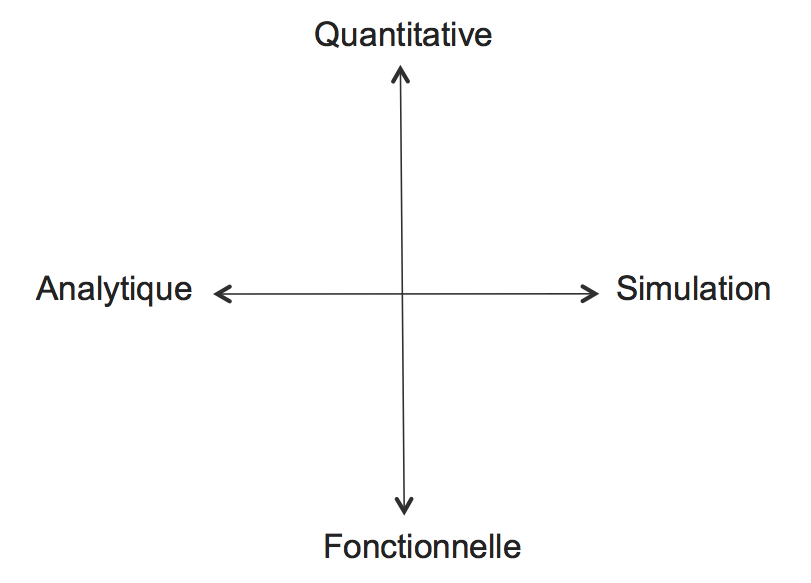
\includegraphics[width=0.75\textwidth]{images/Chapitre1/dimesionsLankhorts.png}
 \end{center}
 \caption{Classification des approches d'analyse selon Lankhorst et al. \protect\cite{lankhorst2009enterprise}}
 \label{fig:classLankhorst}
\end{figure}

La deuxième dimension distingue entre deux techniques pouvant être employées pour l'analyse fonctionnelle ou quantitative~:
	\begin{itemize}
		\item l\textbf{a technique de simulation} des modèles revient à exécuter ces modèles. La simulation dans le cas de l'analyse fonctionnelle est utilisée pour mieux appréhender les aspects dynamiques d'une architecture. La simulation quantitative permet de mesurer de paramètres quantitatifs tel que le temps d'exécution d'un processus métier par exemple à travers différentes itérations de la simulation. 
		\item \textbf{la technique analytique} est plus formelle que la simulation. Ici l'adjectif analytique signifie plutôt «~mathématique~» plus efficace que la simulation quantitative pour fournir des indicateurs de performance.  
	\end{itemize}
	
Ce système de classification offre un premier aperçu des différentes approches d'analyse d'architecture cependant il ne révèle pas toutes les variantes possibles et les subtilités d'une démarche d'analyse en architecture d'entreprise. Nous considérons donc les travaux de Buckl  et al. qui offre un système de classification plus détaillé. Ce système classification peut même être considéré comme un framework d'analyse d'architectures.

Contrairement à Lankhorst et al. \cite{lankhorst2009enterprise}, Buckl et al. \cite{buckl2009classifying} fait appel à cinq dimensions pour catégoriser les approches d'analyse d'architecture. Ces dimensions de classification sont illustrés par la figure~\ref{fig:classBuckl}. Nous les détaillons dans la suite du manuscrit.

\begin{figure}[!htbp]
\begin{tikzpicture}
  \hspace*{-1cm}
  \path[mindmap,concept text=black, level 1/.append style={level distance=4cm}]
    node[concept, scale=0.7] {L'analyse en Architecture d'Entreprise}
    [clockwise from=0]
    child[concept color=black] {
      node[concept, scale=0.9] {Sujet de l'analyse}
      [clockwise from=60]
      child { node[concept, scale=0.9] {Structure} }
      child { node[concept, scale=0.9] {Dynamique} }
      child { node[concept, scale=0.9] {Statistiques} }
    }
    child[concept color=black] {
      node[concept, scale=0.9] {Référence temporelle}
      [clockwise from=-30]
      child { node[concept, scale=0.9] {Ex post} }
      child { node[concept, scale=0.9] {Ex ante} }
    }
    child[concept color=black] { 
    	  node[concept, scale=0.9] {Techniques} 
      [clockwise from=-60]
      child { node[concept, scale=0.9] {Basée sur les experts} }
      child { node[concept, scale=0.9] {À base de règles} }
      child { node[concept, scale=0.9] {À base d'indicateurs} }
    }
    child[concept color=black] { 
      node[concept, scale=0.9] {Préoc\-cupations}
      [clockwise from=-150]
      child { node[concept, scale=0.9] {Fonction\-nelles} }
      child { node[concept, scale=0.9] {Non Fonctionnelles} }
    }
    child[concept color=black] { 
    	  node[concept, scale=0.9] {Auto\-référentialité}
      [clockwise from=-180] 
      child { node[concept, scale=0.9] {Aucune} }
      child { node[concept, scale=0.9] {un niveau} }
      child { node[concept, scale=0.9] {plusieurs niveaux} }      
    }; 
       
\end{tikzpicture}

\caption{Classification des approches d'analyse selon Buckl et al. \protect\cite{buckl2009classifying}}
 \label{fig:classBuckl}
\end{figure}


	\begin{description}
	\item \textbf{Sujet de l'analyse} 

L'analyse se porte sur trois aspects différents de l'architecture~:~sa structure, son comportement dynamique ou son comportement statistique. L'analyse de la structure est nécessaire étant la complexité des entreprises. Celle-ci est due à la densité des interconnexions entres ses composants. La complexité de la structure induit aussi une complexité au niveau de son comportement d'où la nécessité d'analyser l'aspect comportemental de l'architecture pour évaluer l'impact d'une anomalie le déroulement d'un processus par exemple. De plus, l'analyse et l'agrégation des mesures statistiques provenant du comportement offrent une meilleure compréhension de l'architecture.

	\item \textbf{Référence temporelle}

L'architecture peut se porter sur l'architecture d'une entreprise dans son état courant ou telle qu'elle est planifiée. Une analyse ex post concerne les modèles d'une architecture implémentée alors qu'une analyse ex ante se réfère à différents scénarios élaborés pour une futur implémentation.

	\item \textbf{Technique d'analyse}

Les techniques d'analyse peuvent se baser sur des experts, sur des règles ou sur des indicateurs. Les approches d'analyse orientée experts sont les moins formelles dépendent du niveau d'expertise de la personne impliquée et nécessitent plus de temps mais elle sont aussi les plus flexibles. Les résulats d'une telle analyse prennent la forme de conseils concrets ou d'idées générales pour l'architecture en question.

Les techniques d'analyse basées sur des règles sont plus formelles que celles basées sur les experts et peuvent être plus facilement automatisées. Ces règles décrivent des modèles de conceptions que l'architecture doit respecter ou éviter. 

Les techniques d'analyse basées sur des indicateurs sont encore plus formelles que les deux précédentes et servent à évaluer en les quantifiant certaines propriétés de l'architecture. Les résultats d'une telle analyse doivent cependant être interprétés avec prudence. Elle sont en effet basés sur des hypothèses souvent sujettes à évoluer.

	\item \textbf{Préoccupations de l'analyse}

De même que la classification de Lankhorst, Buckl fait la différence entre les analyses fonctionnelles et non fonctionnelles. L'analyse fonctionnelle évalue si l'architecture remplie les fonctions métier de l'entreprise telles la production ou la vente. Il est toutefois aussi important d'évaluer des aspects non fonctionnels tels que le temps d'exécution d'un processus ou le coût de l'implémentation ou de maintenance d'une architecture. Contrairement à Lankhorst, Buckl emploie le terme \textit{non fonctionnelle} plutôt que \textit{quantitative} en arguant que certains aspects non fonctionnels telle que la sécurité peuvent être analysés de manière non quantitative.  

	\item \textbf{Autoréférentialité}
	
Les personnes responsables de l'architecture d'entreprise peuvent faire partie l'architecture créée car elle font aussi partie de l'entreprise. Qui plus est, l'activité de décrire et planifier l'architecture de l'entreprise peut elle-même être décrite et planifiée et fait par conséquent partie de l'activité d'architecture d'entreprise. Selon Buckl \cite{varela1974autopoiesis} l'entreprise est en effet un système vivant capable de faire sa propre autopsie \citep{varela1974autopoiesis}.
L'analyse peut considérer un seul niveau d'autoréférentialité en intégrant les activités de management d'architectures. Une analyse à plusieurs niveaux d'autoréférentialité incorporent des activités de meta-management d'architetcure comme par exemple la gouvernance des activités de management d'architectures.
L'autoréférentialité augmente la complexité d'analyse. Peu de travaux considèrent des niveaux d'autoréférentialité  multiples \cite{smook2014executable}. Nous citons parmis celle-ci les travaux de \cite{metrailler_evolis_2014} qui traitent la gestion et la gouvernance d'architectures notamment en définissant des stratégies d'évolution des architectures actuelles vers les architectures cible dans un framework dédié. 

\end{description}

\subsection{État de l'art de l'analyse en Architecture d'Entreprise} 






\section{Architecture d'entreprise et simulation}
\subsection{approches existantes}

La modélisation c'est pour abstraire
Pour simuler on a besoin de détails



\section{Ingénierie Dirigée par les Modèles}

L'Ingénierie Dirigée par les Modèles (IDM) est née du constat que le paradigme 
du « tout est objet », prôné dans les années 1980, a atteint ses limites avec ce 
début de siècle \cite{greenfield2004software}. En effet, face à la croissance de 
la complexité des systèmes logiciels, au coût de la main d'œuvre et de 
maintenance, une approche centrée sur le code, jugé alors seul représentant 
fiable du système, suscitait de moins en moins l'adhésion des industriels et du 
milieu académique. 

Partant de ce constat, l'Object Management Group (OMG) a proposé en novembre 
2000, l'approche MDA (Model Driven Architecture) qui s'inscrit dans le cadre 
plus général de l'IDM et se réalise autour d'un certain nombre de standards tels 
qu'UML, MOF, XML, QVT, etc. Le monde de la recherche s'y est aussitôt intéressé 
pour dégager les principes fondamentaux de l'IDM 
\cite{bezivin2001towards}\cite{kent2002model} \cite{de2002using} et déjouer le 
piège des définitions parfois trop floues qui prêtent à confusion entre les 
concepts liés aux paradigmes d'objet et de modèle \cite{bezivin2004search}. Par 
ailleurs, des industriels comme IBM \cite{booch2004mda} et Microsoft 
\cite{greenfield2004software} ont aussi rendu publiques leur vision de l'IDM. 
Ainsi, l'IDM prend son origine dans la convergence de toutes ces visions et des 
avancées techniques de chacun.

L'originalité de l'IDM ne réside pas dans le recours systématique aux modèles 
dans le développement logiciel comme le laisserait entendre sa terminologie  
\cite{bezivin2004rapport}. Plusieurs méthodes de modélisation telles que Merise 
ou SSADM préconisent aussi l'utilisation de modèles dont le rôle s'achève aux 
phases amont du développement logiciel : l'analyse et la conception. Les modèles 
servent alors à faciliter la communication et compréhension entre les différents 
acteurs mais n'interviennent pas dans la phase de production, de maintien et 
d'évolution. Nous parlons dans ce cas de modèles « contemplatifs ». 

L'IDM a pour objectif de rendre les modèles « productifs » sur tout le cycle de 
vie du système et à tout niveau d'abstraction. Pour y parvenir, les modèles 
doivent être décrits formellement pour être interprétés et exécutés par une 
machine. Dès lors, ces modèles permettent d'industrialiser la production 
logicielle, jusque-là centrée sur le code produit par l'informaticien 
\cite{bezivin2005unification}.

En mettant à profit des disciplines comme la modélisation par objets, 
l'ingénierie des langages, la compilation de langages, les méthodes formelles, 
la programmation par composants, etc., l'IDM offre un cadre intégrateur reposant 
sur quelques concepts fondamentaux : la notion de modèle et la relation 
\textit{ReprésentationDe}, la notion de métamodèle et la relation 
\textit{ConformeÀ}.

\subsection{Concepts et relations de l'IDM}
\subsubsection{Modèle et ReprésentationDe}
La notion de modèle est centrale dans l'IDM car, comme nous venons de voir, 
l'enjeu de cette approche est de rendre les modèles productifs sur tout le cycle 
de vie du système. Il n'existe pas de définition universelle de la notion de 
modèle. En nous appuyant sur les définitions données dans les travaux 
\cite{minsky1967computation} \cite{bezivin2001towards} et 
\cite{seidewitz2003models}, nous adoptons la définition suivante du terme modèle 
:

\begin{definition}
Un modèle est une abstraction d'un système, selon le bon point de vue, qui 
permet de répondre à des questions prédéfinies sur ce système en lieu et place 
de celui-ci.
\end{definition}

De cette définition découle la première relation fondamentale de l'IDM qui lie 
le modèle et le système qu'il représente. Celle-ci est nommée 
\textit{ReprésentationDe} et notée $(\mu)$. Bien que la relation 
\textit{ReprésentationDe} ne soit pas nouvelle dans l'ingénierie logicielle 
(Merise, UML), l'IDM a permis d'en définir les contours \cite{atkinson2003model} 
\cite{seidewitz2003models} \cite{bezivin2004search}.

\begin{figure}[!htbp]
 \begin{center}
  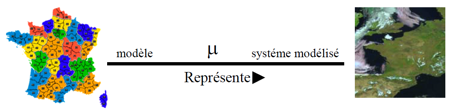
\includegraphics[width=1\textwidth]{images/Chapitre1/favresystememodele.png}
 \end{center}
 \caption{Relation entre système et modèle \protect\cite{favre2006ingenierie}}
 \label{fig:systemModele}
\end{figure}

Cette définition n'est pas restreinte à l'informatique et pourrait s'appliquer à 
n'importe quel système. 
La figure~\ref{fig:systemModele} reprend l'exemple connu de la cartographie où 
une carte géographique joue le rôle de modèle pour une région donnée jouant 
alors le rôle de système modélisé. 

L'intérêt de l'IDM est de produire des modèles exploitables informatiquement. 
Ceci n'est possible que si ces modèles sont décrits par des langages formels. Il 
devient alors important de bien définir ces langages à l'aide de métamodèles

\subsubsection{Métamodèle et ConformeÀ}
L'originalité de l'IDM ne réside pas dans la relation ReprésentationDe qui 
trouve plutôt son origine dans les méthodes de modélisation telles que Merise ou 
SSADM. L'apport de l'IDM est dans l'utilisation systématique de métamodèles pour 
la description des langages de modélisation. 

Il existe plusieurs définitions de la notion de métamodèle dans la littérature. 
Cependant la définition suivante est communément admise 
\cite{bezivin2004rapport}.

\begin{definition}
Un métamodèle est un modèle du langage de modélisation qui sert à exprimer les 
modèles.
\end{definition}
Une autre définition courante mais erronée de la notion de métamodèle suppose 
qu'un métamodèle est un modèle d'un modèle. La figure~\ref{fig:modelofmodel} 
reprend l'exemple de la cartographie évoquée plus haut. Nous appliquons 
récursivement la relation \textit{ReprésentationDe} $(\mu)$ au territoire 
français. Ici une carte de la France joue le rôle de modèle du territoire 
français et un fichier XML joue le rôle de modèle de la carte. Dans ce contre 
exemple, le fichier XML n'est pas un métamodèle de la France. Un métamodèle 
n'est donc pas un modèle d'un modèle.

\begin{figure}[!htbp]
 \begin{center}
  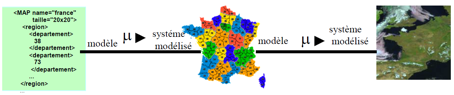
\includegraphics[width=1\textwidth]{images/Chapitre1/modelofmodel.png}
 \end{center}
 \caption{Modèle de modèle selon l'exemple de la cartographie 
\protect\cite{favre2006ingenierie}}
 \label{fig:modelofmodel}
\end{figure}

Par ailleurs, le concept de métamodèle induit la deuxième relation fondamentale 
de l'IDM liant un modèle à son métamodèle. Cette relation est nommée 
\textit{ConformeÀ} et notée $\chi$ \cite{bezivin2004search} 
\cite{favre2004towards}. La figure \ref{fig:carteFavre} reprend l'exemple de la 
cartographie où la légende de la carte joue le rôle de métamodèle ($\chi$) pour 
une carte de la France. En effet, pour être lisible, la carte doit être conforme 
à la légende.

\begin{figure}[!htbp]
 \begin{center}
  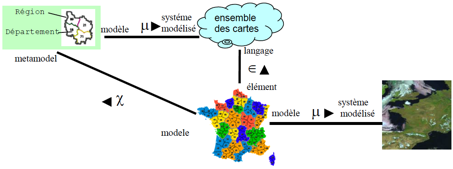
\includegraphics[width=1\textwidth]{images/Chapitre1/cartecompleteIDM.png}
 \end{center}
 \caption{Relations entre système, modèles, métamodèle et langage de 
modélisation \protect\cite{favre2006ingenierie}}
 \label{fig:carteFavre}
\end{figure}

\subsection{Transformation de modèle}
Dans la partie précédente, nous avons introduit les concepts fondamentaux de 
l'IDM que représentent la notion de modèle et la relation 
\textit{ReprésentationDe} ainsi que la notion de métamodèle et la relation 
\textit{ConformeÀ}. Comme expliqué, la préoccupation majeure de l'IDM est de 
rendre les modèles opérationnels sur tout le cycle de vie des systèmes 
logiciels, depuis l'analyse et la conception jusqu'à la maintenance et 
l'évolution. Ainsi, la transformation de modèle se retrouve au cœur de l'IDM car 
c'est à travers elle que se fait l'automatisation des traitements apportés aux 
modèles. Nous allons d'abord donner une définition de la notion de 
transformation de modèle puis en présenter les types et les usages.

\subsubsection{Définition de la transformation de modèle}
L'OMG définit une transformation de modèle comme «~le processus consistant à 
convertir un modèle en un autre modèle d'un même système~» \cite{omg2011meta}. 

\cite{kleppe2003mda} proposent une définition moins générique en insistant sur 
l'aspect automatique de ce processus, ainsi, «~une transformation de modèle 
consiste en la génération automatique d'un modèle source en un modèle cible, 
selon une description établie de cette transformation~». Cette définition 
implique aussi qu'une transformation est décrite à un plus haut niveau 
d'abstraction : au niveau d'un métamodèle auquel elle doit se conformer. 

\cite{mens2006taxonomy} étendent cette définition en considérant qu'une 
transformation est une opération qui peut avoir en entrée un ou plusieurs 
modèles source et en sortie un ou plusieurs modèles cible~: 

\begin{definition}
Une transformation génère automatiquement un ou plusieurs modèles cible à partir 
d'un ou plusieurs modèles source, selon une description établie de la 
transformation. 
\end{definition}

C'est cette dernière définition que nous allons adopter dans ce document. Par 
ailleurs, notons que, si les métamodèles source et cible sont différents, la 
transformation est dite exogène. Si les métamodèles source et cible 
correspondent au même métamodèle, la transformation est dite endogène. Ces 
termes ont été introduits par \cite{mens2006taxonomy}.

\subsubsection{Composants d'une transformation de modèle} 
La figure \ref{fig:composantTransfo} illustre les composants d'une 
transformation de modèle~:~les modèles source, les modèles cible, la définition 
de la transformation et le moteur qui va opérer la transformation selon sa 
définition. 

La description de la transformation spécifie comment un ou plusieurs modèles 
source sont transformés en un ou plusieurs modèles cible. Elle est écrite dans 
un langage de transformation de modèle. Par exemple, si c'est un langage à base 
de règles, la description de la transformation consiste en un ensemble de règles 
de transformation à opérer \cite{kleppe2003mda}. 

Un moteur de transformation exécute ou interprète la description. Il applique 
donc la description aux modèles source pour produire les modèles cible en 
suivant les étapes ci-dessous \cite{tratt2005model}~:

\begin{itemize}
\item Identifier l'élément du ou des modèles source à transformer.
\item Pour chaque élément identifié, produire l'élément cible qui lui est 
associé dans le ou les modèles cible.
\item Produire une trace de la transformation qui lie les éléments du ou des 
modèles cibles aux éléments du ou des modèles source.
\end{itemize}

\begin{figure}[!htbp]
 \begin{center}
   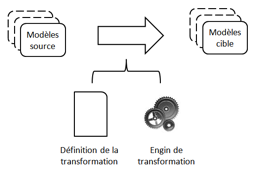
\includegraphics[width=0.7\textwidth]{images/Chapitre1/composanttransfo.png}
 \end{center}
 \caption{Composants d'une transformation de modèle}
 \label{fig:composantTransfo}
\end{figure}

\subsubsection{Usages de la transformation de modèles }
Les transformations de modèles sont au cœur d'une démarche dirigée par les 
modèles~:~elles permettent d'automatiser les manipulations subies par les 
modèles telles que la modification, la création, l'adaptation, la composition ou 
encore le filtrage de modèles, à travers la réutilisation systématique 
d'informations contenues dans les modèles existants. 

Il est possible de recourir aux transformations de modèles sur tout le cycle de 
vie d'un système. Les usages les plus répondus sont le raffinement, 
l'intégration d'outils, la composition, l'analyse, la simulation et 
l'optimisation que nous présentons dans la suite de ce document. 

\begin{description}

\item \textbf{Raffinement}

Le raffinement consiste à rajouter plus de détails au modèle initial. Ce type de 
transformation peut aussi bien être endogène (métamodèles source et cible 
identique) ou exogène (métamodèle source et cible différents). Le raffinement se 
prête parfaitement à toute la partie descendante du cycle en V où les modèles 
passent à des niveaux d'abstraction plus bas. Ceci revient à faire des 
transformations successives de type modèle-à-modèle et une transformation de 
type modèle-à-texte pour aboutir au code final.

Raffiner un modèle revient à décomposer des concepts de haut niveau, à choisir 
un algorithme particulier, à spécialiser un concept pour un contexte donné ou 
encore à le concrétiser sous forme d'une solution exécutable par une machine en 
générant le code à partir de modèles de plus haut niveau d'abstraction 
\cite{czarnecki2000intentional}. 

\item \textbf{Intégration d'outil}

Il existe une panoplie d'outils disponibles pour créer, manipuler, analyser ou 
encore simuler des modèles. Souvent ces outils utilisent des métamodèles 
internes et des espaces techniques qui leurs sont propres. Ainsi, l'échange de 
modèle entre ces outils est compromis et l'interopérabilité est fortement 
entravée. L'utilisateur se trouve obligé d'utiliser un seul et même outil sur 
tout le cycle de vie du système et ne peut donc pas tirer avantage des 
possibilités offertes par d'autres outils plus adaptés à ses besoins à certaines 
étapes.

L'intégration d'outil est une solution pour palier la divergence syntaxique et 
sémantique des outils et des langages de modélisation par le biais la 
transformation de modèle \cite{tratt2005model}. Ce type de transformation permet 
de naviguer entre deux métamodèles, de synchroniser des modèles qui évoluent 
séparément sur des outils distincts, de faire des mapping entre métamodèles pour 
maintenir la cohérence des modèles conformes à ces métamodèles. Il sera donc 
possible de faire appel à des outils mieux adaptés à chaque étape du cycle de 
vie.

\item \textbf{Composition}

Pour réduire la complexité inhérente à la modélisation et à l'analyse de grands 
systèmes, tels que les Smart Grids par exemple, il est possible d'adopter une 
approche par points de vue qui permet de séparer les préoccupations. Les modèles 
produits correspondent donc à ces différents points de vue qu'on peut ainsi 
valider séparément dans un premier temps. A l'issue de cette approche modulaire, 
on pourra composer ces modèles, c'est-à-dire les assembler, pour aboutir un 
modèle global du système.

Dans le cas le plus simple, les deux modèles à composer sont conformes à un même 
métamodèle. Cependant, il est aussi possible de composer deux modèles conformes 
à deux métamodèles différents. 

Les deux modèles à composer peuvent aussi présenter des concepts en commun. Deux 
techniques existent pour composer des modèles, que nous illustrons dans la 
figure \ref{fig:compoExemple}~:

\begin{itemize}
\item La première technique consiste à les fusionner. Dans ce cas, le modèle 
final résultant de la composition doit contenir toutes les informations issues 
des modèles initiaux, sans duplication des informations communes 
\cite{bezivin2006canonical}.
\cite{fleurey2008generic} présente un framework générique capable de composer 
des modèles indépendamment de leurs langages de modélisation. L'approche 
consiste à identifier les éléments qui représentent le même concept dans les 
deux modèles à composer et à les fusionner dans un nouveau modèle qui représente 
une vue intégrée de ces concepts. Il est aussi possible de spécialiser le 
framework pour un métamodèle particulier mais qui reste conforme au MOF.

\item La deuxième technique consiste à les tisser. Dans ce cas, on crée des 
correspondances entre les éléments qui représentent un même concept. Un 
métamodèle générique est créé pour définir les correspondances qui sont donc 
modélisées dans le modèle final. On y retrouve donc les éléments en commun 
dupliqués mais liés par un lien de correspondance. 
\end{itemize}

Il est à noter que le modèle issu du tissage de deux modèles $M_{A}$ et $M_{B}$ 
peut être utilisé comme modèle intermédiaire que l'on note $M_{T}$ pour la 
fusion de $M_{A}$ et $M_{B}$. Dans ce cas L'opération de fusion consiste à 
produire un modèle $M_{AB}$ en prenant comme entrée $M_{A}$, $M_{B}$ et $M_{T}$. 
Cette technique est notamment utilisée par \cite{del2007semi} pour la 
composition semi-automatique de modèles.

\begin{figure}[!htbp]
 \begin{center}
  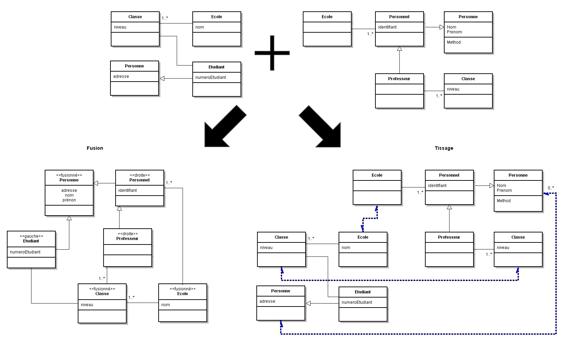
\includegraphics[width=1\textwidth]{images/Chapitre1/compoExemple.png}
 \end{center}
 \caption{Exemple de composition de deux modèles}
 \label{fig:compoExemple}
\end{figure}

\item \textbf{Simulation}

La transformation de modèle peut être utilisée pour simuler des modèles. En 
effet, une transformation de modèle peut mettre à jour le système modélisé. Dans 
ce cas, le modèle cible est une mise à jour du modèle source et la 
transformation est de type sur-place (modèles source et cible confondus). 

Par exemple, \cite{syriani2011multi} simule un comportement simple d'un jeu de 
Pacman en utilisant la transformation de modèle. La transformation spécifie les 
règles de transition qu'une instance du jeu peut prendre (Pacman et fantôme se 
trouvant dans la même case, Pacman et pomme se trouvant dans la même case, 
etc.). En ingénierie des langages, ceci revient à définir la sémantique 
opérationnelle d'un langage de modélisation. L'exécution de la transformation 
anime le modèle en fonction du comportement qu'on lui confère.

La transformation peut aussi être utilisée comme intermédiaire dans la 
simulation de modèle. Des modèles en entrée d'un outil de simulation externe 
sont produits par une transformation des modèles qu'on souhaite simuler. Cette 
technique permet de tirer profit d'outils de simulation existant sur le marché 
en utilisant l'intégration d'outils.

\item \textbf{Analyse et optimisation}

La transformation de modèle peut être utilisée pour les activités d'analyse de 
modèle. Une analyse simple telle que le calcul de métrique de similarité entre 
deux modèles via la transformation de modèle est donnée dans \cite{del2007semi} 
avec un modèle de transformation écrit en ATL \cite{jouault2006transforming}. 

Des analyses plus complexes sont possibles grâce à l'intégration d'outils 
d'analyse externes vers lesquels les modèles source sont transformés.

\cite{biehl2010integrating} propose d'utiliser la transformation de modèle pour 
l'analyse de sûreté de fonctionnement dans le domaine de l'automobile. Les 
modèles source sont transformés en modèles conformes au métamodèle de l'outil 
d'analyse de sûreté de fonctionnement retenu.
 
L'optimisation vise à améliorer les propriétés non fonctionnelles des modèles 
telle que l'évolutivité, la fiabilité, la modularité, etc. L'optimisation est 
typiquement utilisée sur les modèles d'architecture. Les transformations 
utilisées pour l'optimisation sont de types endogènes car on cherche à affiner 
la conception de modèles existants. La réingénierie est un exemple de 
transformation utilisée pour optimiser les modèles~:~on cherche à améliorer la 
maintenabilité, la lisibilité et l'évolutivité des modèles.

\end{description}

\subsubsection{Approches existantes pour la transformation de modèle}  
Le recours à la transformation de modèle est l'objet de recherches informatiques 
antérieures à l'apparition de l'approche IDM. Par exemple, les compilateurs 
utilisent la transformation pour passer du code source au fichier binaire 
\cite{aho1985compilers}. Ce type de transformation est restreint au domaine de 
la programmation informatique. La transformation de modèle embrasse un domaine 
plus large encore.

Nous trouvons dans la littérature plus d'une trentaine d'approches différentes 
de transformation de modèle \cite{syriani2011multi}. Czarnecki et Helsen 
proposent une classification de ces approches selon plusieurs critères tels que 
le paradigme retenu pour définir la transformation, la relation entre les 
modèles sources et cibles, la directivité de la transformation, le nombre de 
modèles cible et source, l'orchestration et l'ordonnancement des règles de 
transformation, etc. \cite{czarnecki2006feature}.

\cite{blanc2011mda} retient trois grandes catégories d'approches~:

\begin{itemize}
\item Par programmation

Les modèles offrent une interface qui permet d'écrire les transformations dans 
un langage de programmation. Mais cette technique relève plus de la 
programmation que de la modélisation. Ce sont en fait des applications 
informatiques qui ont la particularité de manipuler des modèles. L'avantage de 
cette approche est que l'on utilise un langage de programmation généraliste tel 
que Java ou C++ pour écrire les transformations. Ainsi le programmeur n'a pas 
besoin d'apprendre un nouveau langage. Cependant ces applications ont tendance à 
devenir difficilement maintenables. 

\item Par template 

Dans cette approche on définit des canevas des modèles cibles. Ces modèles 
contiennent des paramètres qui seront remplacés par les informations contenues 
dans les modèles source. Ce type de transformation est souvent utilisé pour les 
transformations modèle-à-texte et est associé au visitor-pattern qui va 
traverser la structure interne du modèle source. Cette approche est utilisée par 
l'outil Enterprise Architect par exemple. 

\item Par modélisation

Cette approche vise à appliquer les principes de l'IDM aux transformations de 
modèles elles-mêmes. Ainsi, on produit des modèles de transformation prennes, 
réutilisables et indépendants des plates-formes d'exécution 
\cite{bezivin2006model}. 

Pour cela, on utilise des langages de modélisation dédiés à l'activité de 
transformation de modèles. Cette approche considère donc la transformation comme 
un modèle à part entière conforme à un métamodèle de transformation. La figure 
\ref{fig:TransfoPrincipe} , illustre cette approche en positionnant la 
transformation sur les différents niveaux d'abstraction de l'IDM. Elle corrobore 
ainsi la vision unificatrice de l'IDM à travers le paradigme du « tout est 
modèle » \cite{bezivin2005unification}. Le langage de transformation ATL, que 
nous présentons dans la section~\ref{sec:ATL}, a été développé dans ce sens. 

\end{itemize}

\begin{figure}[!htbp]
 \begin{center}
  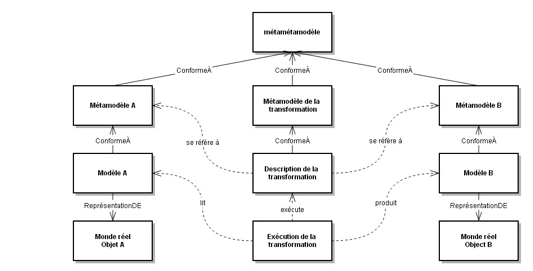
\includegraphics[width=1\textwidth]{images/Chapitre1/transfoPrincipe.png}
 \end{center}
 \caption{Méta niveaux d'une transformation de modèle}
 \label{fig:TransfoPrincipe}
\end{figure}

\subsection{Langages et outils pour la transformation de modèle}
Dans cette section, nous introduisons succinctement quelques langages et outils 
dédiés à la transformation de modèles, sans viser à l'exhaustivité.

\subsubsection{ATL}
\label{sec:ATL}
Atlas Transformation Language (ATL) \cite{jouault2006transforming} 
\cite{jouault2008atl} est né de la volonté de proposer des langages de 
modélisation dédiés à la transformation de modèle en définissant un métamodèle 
et des outils pour l'exécution des transformations. Il permet de réaliser des 
transformations de type modèle-à-modèle et de type modèle-à-texte.

ATL  est un langage hybride (déclaratif et impératif) à base de règles OCL (OMG 
2014). Une règle déclarative, appelée Matched rule, permet de décrire 
l'implémentation de mapping simples entre les modèles source et cible en 
utilisant des patrons source (\textit{InPattern}) mappés avec les éléments 
source et des patrons cibles (\textit{outPattern}) mappés avec les éléments 
cible. 

L'approche impérative explicite les étapes d'exécution de la transformation à 
travers les Helpers. Ce mécanisme de Helpers permet en outre d'éviter la 
redondance de code et la création de longues règles écrites en OCL, ce qui 
confère une meilleure lisibilité aux programmes ATL. 

Une transformation écrite en ATL est composée d'un ensemble de règles qui 
spécifient comment créer et initialiser les éléments des modèles cible. Il n'est 
pas possible de spécifier l'ordre d'exécution des règles de transformation. Cet 
ordre est établi automatiquement, exception faite pour les \textit{lazy rules} 
qui ont besoin qu'on fasse spécifiquement appel à elles. ATL est conforme au 
méta-métamodèle MOF et est doté d'une syntaxe concrète textuelle. Il est intégré 
à l'environnement Eclipse. Une transformation prend en entrée un ensemble de 
modèles conformes à Ecore (EMF 2014) ou KM3 \cite{jouault2006km3}.

ATL ne prend pas en charge les transformations incrémentales. Il commence par 
lire entièrement les modèles source et génère des modèles cible complet. Les 
modifications manuelles dans les modèles cible ne sont donc pas préservées si 
l'on opère une nouvelle transformation.

ATL peut réaliser des transformations sur  place, c'est-à-dire, une 
transformation où le modèle source et le modèle source sont confondus en 
utilisant le mode raffinement de modèle. Cependant ce mode présente quelques 
limitations avec certaines fonctionnalités comme celle des \textit{lazy rules}.

\subsubsection{QVT}
Le framework Query View Transformation (QVT) \cite{kurtev2008state} 
\cite{omg2011meta} a rejoint la batterie de standards de l'OMG. Le métamodèle de 
QVT est conforme au MOF. Comme ATL, QVT se base sur OCL pour accéder aux 
éléments des modèles.
QVT définit trois langages de transformation de type modèle-à-modèle. 
QVT-Relations (QVT-R) et QVT-Core (QVT-C) sont des langages déclaratifs qui 
adressent deux niveaux d'abstraction différents. QVT-Operational Mappings 
(QVT-OM) est un langage impératif qui étend QVT-R et QVT-C.

QVT-R est un langage de transformation de haut niveau d'abstraction doté de 
syntaxes concrètes textuelle et graphique. Les transformations, 
bidirectionnelles, sont spécifiées sous forme de relations entre les modèles 
source et cible. Une transformation a pour but de vérifier la cohérence entre 
deux modèles, renforcer la cohérence en modifiant le modèle cible, synchroniser 
deux modèles ou encore pour raffiner un modèle par une transformation sur-place. 
La sémantique de QVT-R est définie par une transformation vers QVT-C.

QVT-C est un langage de transformation de bas niveau qui sert de base pour 
QVT-R. Les deux ont le même niveau d'expressivité. Une transformation consiste 
en la déclaration de mapping entre les métamodèles source et cible en utilisant 
des patterns. Contrairement à QVT-R, la traçabilité est explicitement définie à 
travers les liens entre les métamodèles.

QVT-OM est un langage de transformation impératif qui étend QVT-R avec des 
constructions impératives basée sur une extension impérative de OCL. Les 
transformations sont unidirectionnelles mais établissent explicitement des 
modèles de traçabilité.

QVT est aussi doté d'un mécanisme de \textit{graybox} qui permet de faire appel 
à des algorithmes complexes écrits dans n'importe quel langage de programmation 
et d'utiliser des librairies existantes. Mais ce mécanisme rend la 
transformation opaque puisqu'il n'est pas contrôlé par le moteur d'exécution. 
Nous pouvons citer SmartQVT ou encore ModelMorf comme machines d'exécution de 
transformation écrite en QVT.

\subsubsection{Kermeta}
Kermeta est un langage généraliste de méta-modélisation exécutable et de 
méta-programmation orientée objet qui peut aussi décrire des transformations de 
modèle. Intégré à EMF, il est doté d'un métamodèle conforme au MOF qu'il étend 
avec un langage d'action impératif utilisé pour écrire le corps des opérations 
définies sur les concepts d'une syntaxe abstraite (ce qui revient à doter une 
syntaxe abstraite d'une sémantique opérationnelle). On peut ainsi décrire 
n'importe quel traitement sur un modèle ce qui est assimilé à une transformation 
de modèle.

Le langage d'action de Kermeta permet d'écrire des expressions impératives qui 
spécifient explicitement la construction des éléments des modèles cible. A 
l'inverse de QVT-OM, Kermeta n'est pas un langage à base de règles.  
Kermeta est capable de gérer les exceptions mais les transformations 
multidirectionnelles ne sont pas supportées par les outils d'exécution. Il en 
est de même pour la transformation incrémentale. Les modèles source sont lus en 
une seule fois et les modèles cible sont produits complets lors de l'exécution 
de la transformation.





    \appendix
%    \chapter{Investigations pour la vue métier}
\label{annexe:DataSimu}

\section{Exemple d'annexe}

.
    \bibliographystyle{plain}
    \bibliography{bibliography}
\end{document}
